\chapter{Introduction}

\noindent\hfill\parbox{0.85\textwidth}{\raggedleft
\QuoteBy{I saw the best minds of my generation destroyed by madness, \dots angle-headed hipsters burning for the ancient heavenly connection to the starry dynamo in the machinery of night, \dots}{``Howl'' by Allen Ginsberg (1955)}
}\par

\vspace{1.5 cm}

\section{A Dynamical View of Galactic Magnetism}

While a galaxy's mass is largely concentrated in stars, planets, and black holes, most of its volume is filled by diffuse gas. Moreover, this gas is largely ionised and therefore in a plasma state, where a sea of electrons and ions can drift relative to one another; this relative drift drives electric currents, which in turn generate magnetic fields. Magnetic fields are therefore a natural consequence of plasma dynamics in galaxies, and unlike collisional gas interactions, allow plasmas to influence parts of flows far from where currents are produced. While these fields are not visible to our eyes, we have techniques that can reveal them (see \S\ref{sec:how-we-see}), and have shown that they not only thread an enormous range of scales in galaxies, from star-forming regions to large-scale outflows, but are already present in the first galaxies (see \S\ref{sec:what-we-see}).

The plasma conditions of galaxies have evolved over cosmic time (see \S\ref{sec:evolve}), so the magnetic fields we infer today are unlikely to resemble primordial seed fields (see \S\ref{sec:modelling:magnetogenesis}). Instead, the first fields are believed to have been amplified and reorganised as galaxies assembled, through a process that is best described within the magnetohydrodynamic (MHD; see \S\ref{sec:modelling:mhd}) formalism.

In the remainder of this introduction we provide a broad overview of the observations and theory that are relevant to this thesis. We begin by describing how magnetic fields are inferred in and around galaxies, and then turn to the dynamical processes that amplify and reorganise these fields. We close this introduction in \S\ref{sec:intro:roadmap}, by framing the questions tackled in this thesis against this background.

\section{Evidence Our Universe is Magnetised}
\label{sec:magnetised-universe}

\subsection{How we reveal the invisible}
\label{sec:how-we-see}

While magnetic fields do not emit radiation directly, their presence can be inferred from the imprint they leave on radiation that has been emitted by and propagated through ionised environments. This inference rests on physics established through laboratory experiments and near-Earth space measurements, which have revealed how magnetic fields influence charged particles and how they modify the polarisation and spectral properties of the radiation we observe. In astrophysics, these same signatures are used to probe and constrain properties of magnetic fields in distant systems, where entire observational surveys are often built around employing a single technique. The catch, however, is that each probe is only sensitive to a particular component of the field, and moreover, the inferred signal is often also impacted by other properties of the medium. Therefore no single observational technique is able to provide a complete view of the cosmic magnetism that threads our Universe. Instead, a coherent picture only emerges once we combine complementary measurements, with the degeneracies of one tracer constrained by another.

Below we discuss a number of observational techniques, highlighting the conditions under which they are useful and which components of magnetic fields they reveal (summarised in \autoref{table:seeing:reqs} and \ref{table:seeing:b-parts}). We then highlight some of the galactic magnetic-fields inferred using these probes in \S\ref{sec:what-we-see}.

\begin{table}
\centering
\caption{Summary of the conditions required for the observational probes discussed below, to produce signatures of cosmic magnetic fields.}
\label{table:seeing:reqs}
\renewcommand{\arraystretch}{1.65}
\begin{tabular}{>{\raggedright\arraybackslash}p{0.3\textwidth} p{0.65\textwidth}}
    \hline
    Probe & Environmental requirements (and limitations) \\
    \hline
    Zeeman splitting (\S\ref{sec:how-we-see:zeeman})
    & Atomic or molecular transitions with narrow, bright spectral lines \\

    Synchrotron radiation (\S\ref{sec:how-we-see:synchrotron})
    & Relativistic electron population; sensitive to beam averaging \\

    Faraday rotation (\S\ref{sec:how-we-see:faraday-rotation})
    & Ionised medium with free electrons along the line of sight; polluted by foreground contamination \\

    Dust polarisation (\S\ref{sec:how-we-see:polarisation})
    & Dust grains in an anisotropic radiation field; affected by line-of-sight and beam averaging \\
    \hline
\end{tabular}
\end{table}

\begin{table}
\centering
\caption{Summary of observational probes and the magnetic field components that they constrain.}
\label{table:seeing:b-parts}
\renewcommand{\arraystretch}{1.65}
\begin{tabular}{>{\raggedright\arraybackslash}p{0.325\textwidth} p{0.625\textwidth}}
    \hline
    Magnetic field component & Observational sensitivity \\
    \hline
    Total field strength, $b$
    & Synchrotron intensity (\S\ref{sec:how-we-see:synchrotron}; indirect; depends on particle population and assumptions, \eg equipartition) \\

    Plane-of-sky field, $b_\perp$
    & Synchrotron polarisation (\S\ref{sec:how-we-see:synchrotron}); dust polarisation (\S\ref{sec:how-we-see:polarisation}; orientation; strength inferred via the Davis-Chandrasekhar-Fermi method) \\

    ``Ordered'' vs ``turbulent'' field structure
    & Synchrotron (de)polarisation (\S\ref{sec:how-we-see:synchrotron}); beam and line-of-sight averaging (\S\ref{sec:how-we-see:polarisation}) \\

    Line-of-sight field, $b_\parallel$
    & Faraday rotation (\S\ref{sec:how-we-see:faraday-rotation}; weighted by thermal electrons); Zeeman splitting (\S\ref{sec:how-we-see:zeeman}) \\

    Large-scale field  coherence
    & Variation of Faraday rotation across sightlines (\S\ref{sec:how-we-see:faraday-rotation}); similarly for polarisation (\S\ref{sec:how-we-see:synchrotron}, and \S\ref{sec:how-we-see:polarisation}) \\

    Small-scale field fluctuations
    & Depolarisation, beam averaging, and frequency-dependent Faraday effects (\S\ref{sec:how-we-see:faraday-rotation}); beam and line-of-sight averaging (\S\ref{sec:how-we-see:synchrotron}, \S\ref{sec:how-we-see:polarisation}) \\
    \hline
\end{tabular}
\end{table}


\subsubsection{Zeeman Splitting}
\label{sec:how-we-see:zeeman}

Zeeman splitting provides one of the most direct ways to measure astrophysical magnetic fields \citep{crutcher2012magnetic, crutcher2019review}. It relies on detecting the Zeeman effect in spectral lines, which is caused by an external magnetic field shifting the energy levels of ions, atoms, or molecules, which leaves a corresponding imprint on the observed spectrum. When detected, this directly constrains the line-of-sight component of the field, $b_\parallel$, which, in contrast to the other probes we discuss below, does not hinge on any assumptions about cosmic-ray populations or energy equipartition, and instead depends directly on the local magnetic field (where the emission took place) \citep{crutcher2012magnetic}; the observed signal is illustrated in \autoref{fig:zeeman}.

\begin{figure}
    \centering
    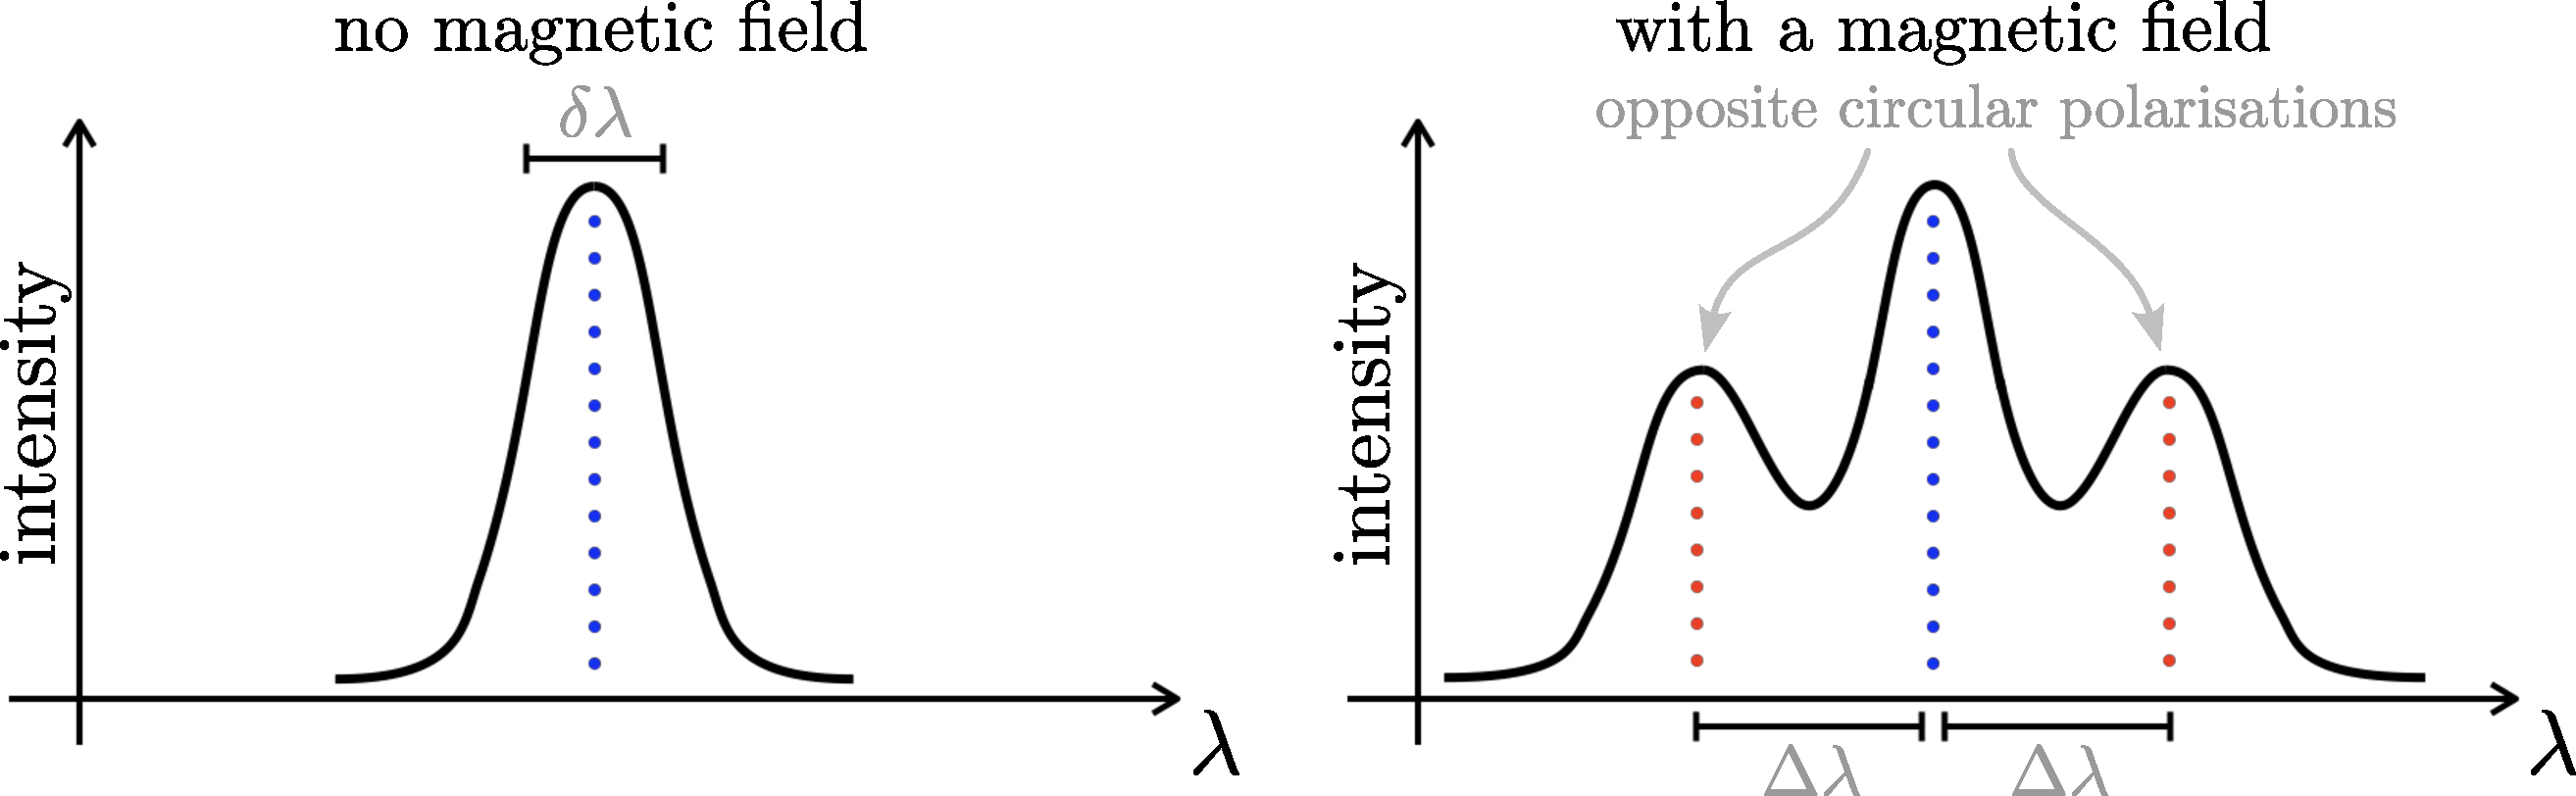
\includegraphics[width=\linewidth]{figures/introduction/zeeman.pdf}
    \caption{Schematic of Zeeman splitting in a spectral line. Without a magnetic field (left), a transition produces a single line with characteristic width $\delta\lambda$ set by thermal and turbulent Doppler broadening. In the presence of a magnetic field (right), the line splits into components with different circular polarisations that are shifted in frequency by $\Delta\lambda \propto b_\parallel$, where $b_\parallel$ is the line-of-sight component of the field. In this figure I have exaggerated the size of the shift for visiblity, but in practice in the interstellar medium, the shift $\Delta\lambda$ is almost always smaller than the intrinsic linewidth $\delta\lambda$, and thus the shift is detected by detecting a residual after differencing the two polarisation components.}
    \label{fig:zeeman}
\end{figure}

This effect arises as a consequence of electrons carrying magnetic moments associated with their spin and orbital motion. In the absence of an external magnetic field, these moments have no preferred orientation, so the magnetic sublevels relevant to a given transition are degenerate, and the transitions only produce spectral lines at a single frequency. However, when an external magnetic field is present, the field couples to the magnetic moments of bound electrons in the emitting or absorbing species, and exerts a torque that causes them to precess about the field's orientation. In these configurations, the field favours orientations that are more closely aligned or anti-aligned, which lifts the degeneracy and shifts the corresponding transition's energy levels by a small amount. In turn, these energy shifts translate into small frequency offsets,
\begin{align}
    \Delta \lambda
        \propto b_\parallel
    ,
\end{align}
in the emitted or absorbed radiation.

Despite its apparent simplicity, Zeeman splitting is not trivial to apply in astronomy \citep[see details by \eg][]{brauer2017magnetic}. This is because the magnitude of the splitting, $\Delta \lambda$, depends on the transition's Zeeman coefficient (set by its effective Land\'e factor), so only a small set of species provide sufficiently large Zeeman sensitivity. In the interstellar medium, where magnetic fields are typically quite weak (at least compared to the plasma environments we can create in laboratories on Earth), this limits us to tracers like the atomic hydrogen 21-cm transition and molecules with large electronic magnetic moments, like OH, CN, CH, CCS, SO, and O$_2$. However, even for these tracers, $\Delta \lambda$ is usually much smaller than the observed line width $\delta \lambda$ set by thermal (and turbulent) Doppler broadening, so the Zeeman components are rarely resolved as separate peaks.

In practice, one therefore measures the associated circular-polarisation signature across the line profile. The split Zeeman components carry opposite circular polarisations, so splitting the signal into left- and right-circular polarisations and differencing them yields a characteristic antisymmetric residual whose amplitude is proportional to $b_\parallel$. Because many instrumental and sky-noise contributions enter both polarisation channels in a similar way, differencing suppresses the shared noise-modes and allows detection of much weaker splitting than would be possible from total intensity alone. Where it can be applied, Zeeman splitting provides a uniquely direct constraint on $b_\parallel$, which can be used to calibrate and validate field estimates inferred from synchrotron emission and Faraday rotation.

\subsubsection{Synchrotron Radiation}
\label{sec:how-we-see:synchrotron}

At radio wavelengths, synchrotron radiation from relativistic electrons provides one of the most widely used tracers of cosmic magnetism \citep{vallee2011magnetic}. As these electrons propagate through magnetised environments, their trajectories are bent by magnetic tugs (the Lorentz force) into gyrating trajectories about magnetic field lines. Since these particles experience a constant acceleration, they radiate, and since they are relativistic, their radiation is strongly beamed along the instantaneous direction of motion. An ensemble of gyrating electrons then produces diffuse radiation whose intensity depends on the magnetic field strength, $b$, and on the energy distribution of the radiating electrons, while its polarisation traces the geometry of the plane-of-sky component, $b_\perp$. \autoref{fig:synchrotron} illustrates the basic geometry of this process.

\begin{figure}
    \centering
    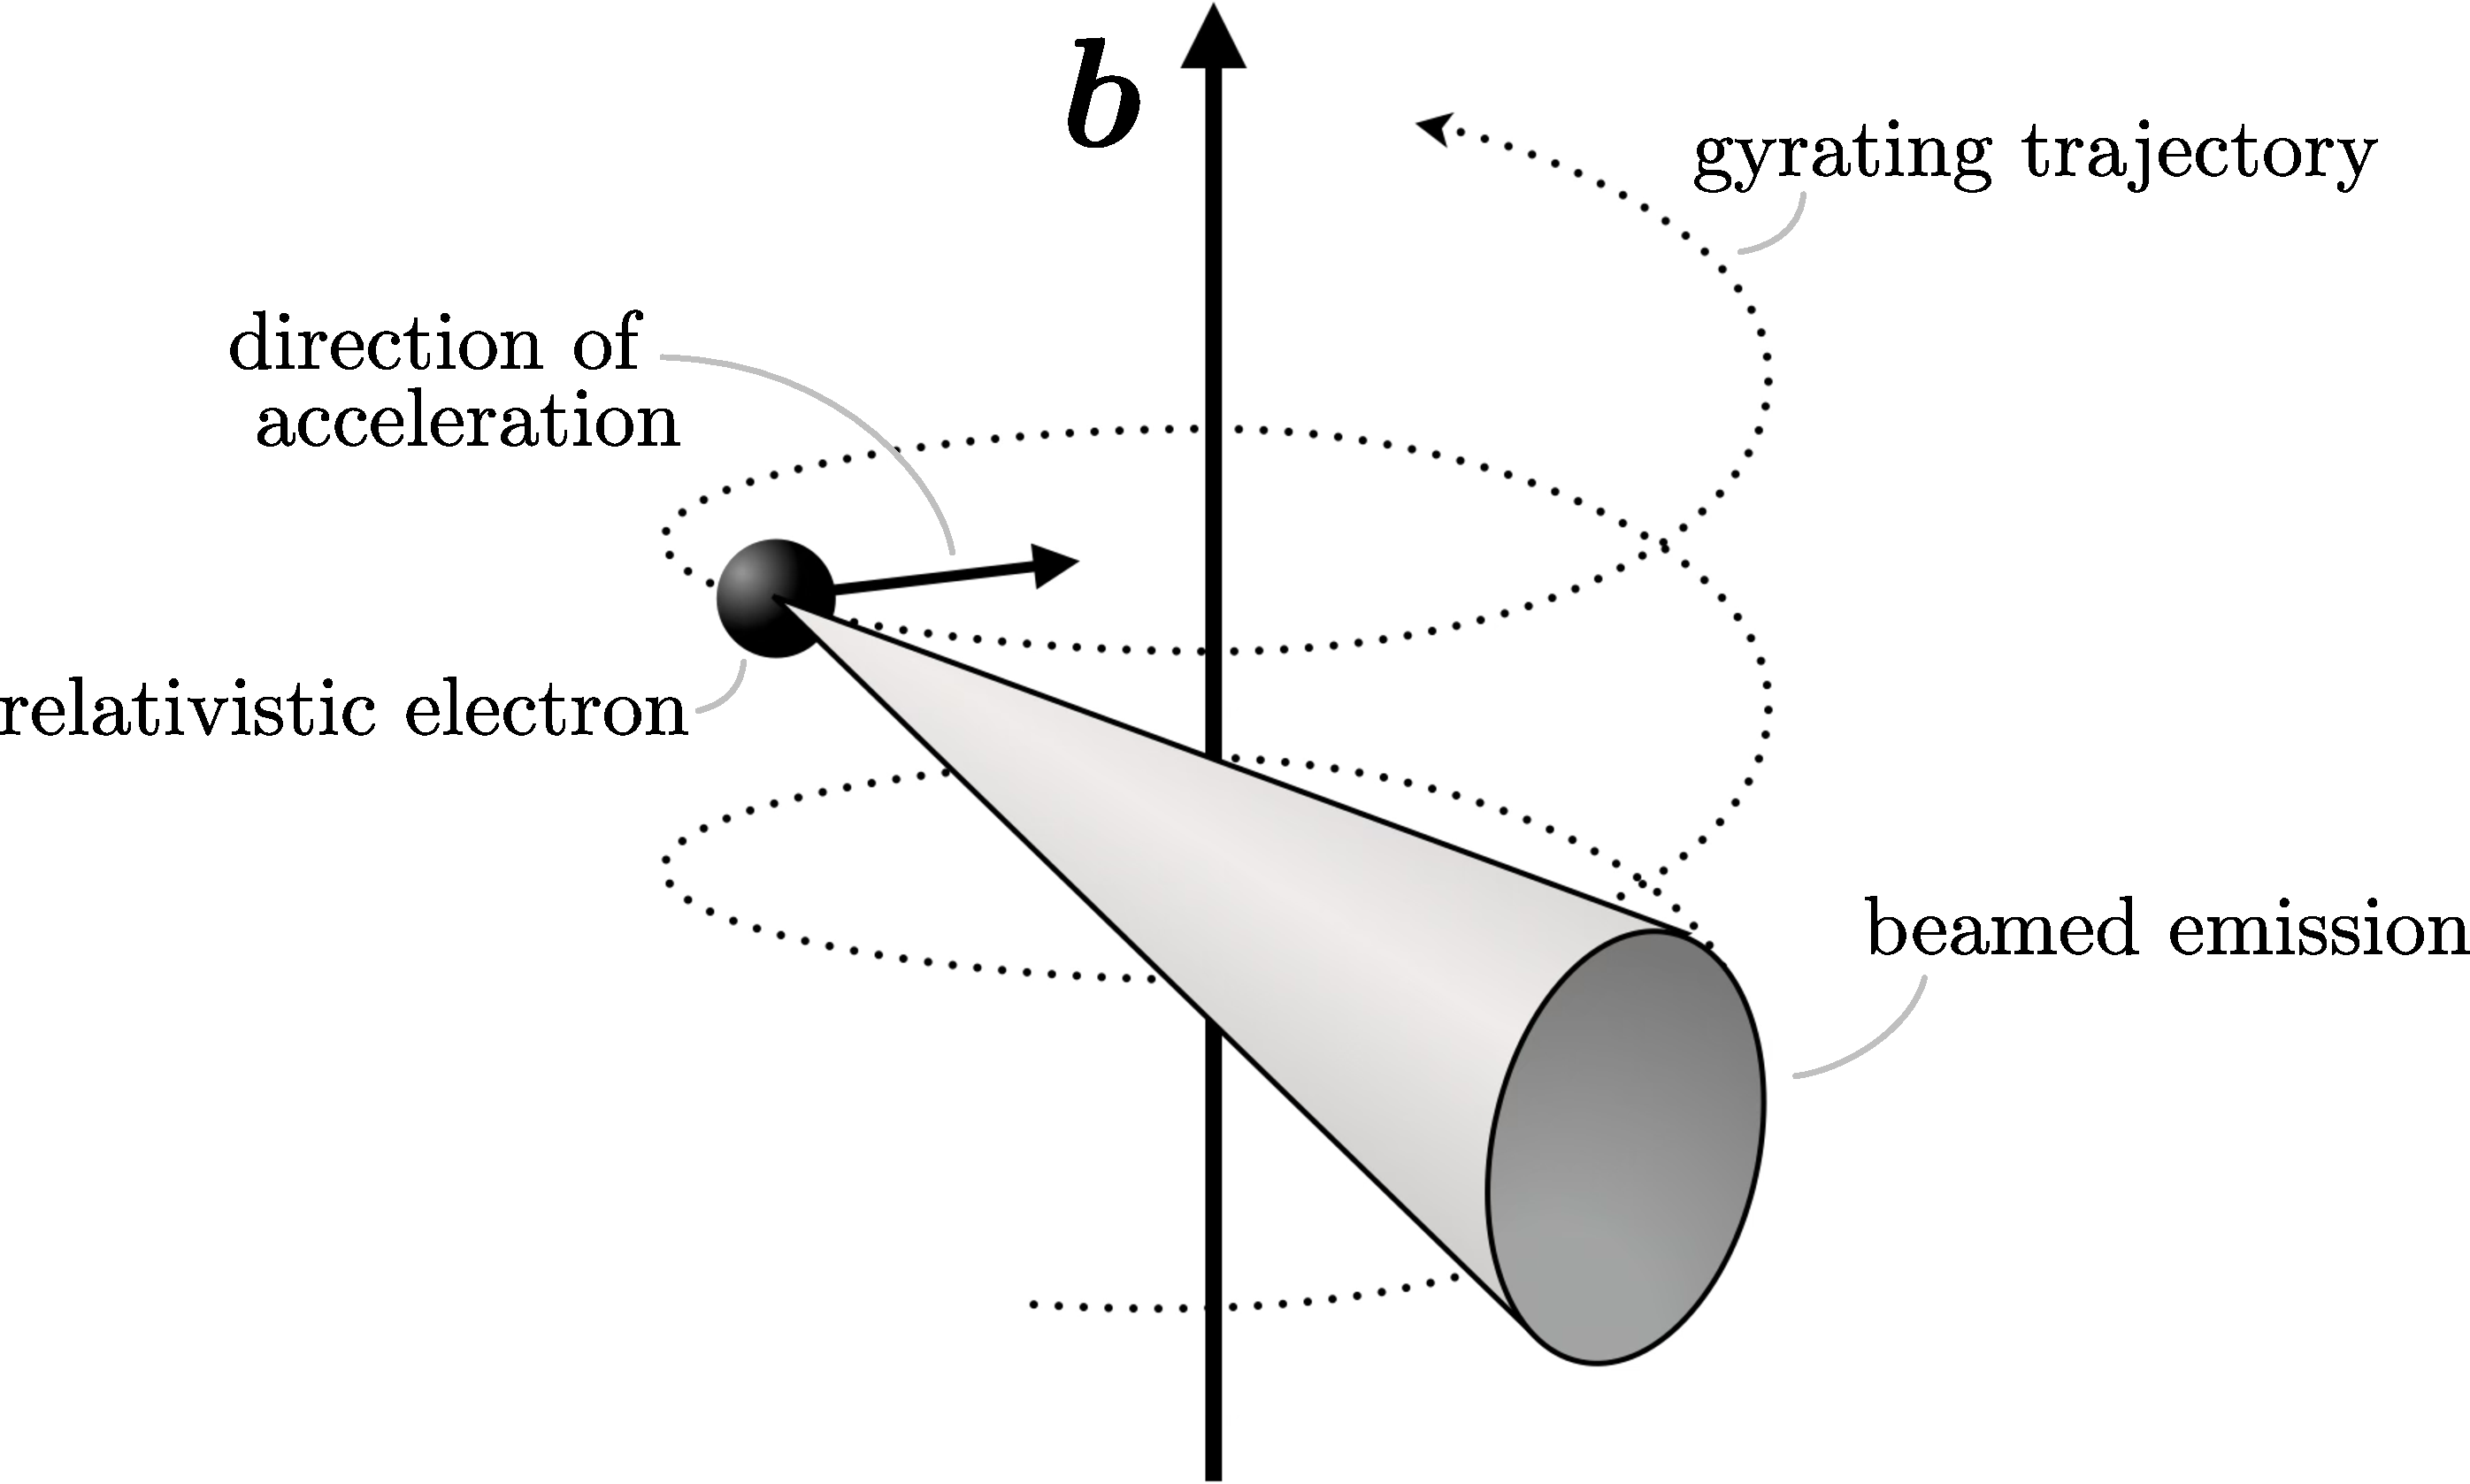
\includegraphics[width=0.85\linewidth]{figures/introduction/synchrotron.pdf}
    \caption{Schematic of synchrotron emission, adapted from \citet{shukurov2021astrophysical}. A relativistic electron gyrates about a magnetic field, $\mVector{b}$, with the Lorentz force providing an acceleration directed toward the local centre of its trajectory. Because the electron is relativistic, the emitted radiation is strongly beamed along the instantaneous direction of motion, producing a narrow emission cone.}
    \label{fig:synchrotron}
\end{figure}

At longer radio wavelengths ($\lambda \sim \mathrm{cm}-\mathrm{m}$), synchrotron emissivity depends on the relativistic electron population and the magnetic field strength,
\begin{align}
    \epsilon_\lambda
        \propto n_\mathrm{re}\, b^{(p+1)/2}\, \lambda^{(p-1)/2}
    ,
\end{align}
for an electron energy distribution $\mdd n / \mdd E_e \propto E_e^{-p}$, where $n_\mathrm{re}$ is the relativistic electron number density, and $p$ is the electron spectral index. Synchrotron emission therefore constrains $b$ only in combination with $n_\mathrm{re}$. The intensity alone cannot be inverted to a magnetic field strength without a closure for $n_\mathrm{re}$ (or, more generally, for the cosmic-ray electron energy density). However, a common closure, and perhaps the simplest choice, is to assume an approximate equipartition between the energy densities of cosmic rays and magnetic fields \citep{beck2005revised}, which yields a practical estimate of $b$, but inherits uncertainty from assumptions about the particle spectrum, filling factors, and the degree to which local energy balance holds true \citep{seta2019revisiting}.

Synchrotron emission is intrinsically linearly polarised, and so polarisation angle provides a second observable probe, alongside the total intensity, revealing the orientation of the ordered component of $b_\perp$. That said, the measured angle is not, in general, the same as the emission angle, because propagation through a magnetised plasma can rotate the plane of polarisation (see Section~\ref{sec:how-we-see:faraday-rotation}). Moreover, the polarisation fraction is also often suppressed, since the observed signal could contain many emitting regions along the line-of-sight (and across the telescope beam), so polarisation contributions may partially cancel. Polarisation, therefore, tends to mainly diagnose the degree of ordering in $b_\perp$, but cannot by itself tell whether the ordered component reflects a truly coherent field, or an anisotropically aligned, turbulent one.

At higher energies, relativistic electrons can also produce X-ray emission through inverse Compton scattering, which in some environments provides a useful complement to synchrotron measurements. For example, in radio-galaxy lobes (where seed photons are dominated by the cosmic microwave background) and in compact hotspots (where synchrotron self-Compton emission can apply), magnetic field strengths can be constrained from the ratio of synchrotron to inverse-Compton flux \citep[see reviews by \eg][]{worrall2002gaseous, hardcastle2020radio}.

\subsubsection{Faraday Rotation}
\label{sec:how-we-see:faraday-rotation}

Faraday rotation probes magnetic fields through their effect on the propagation of linearly polarised radiation, and explains why the polarisation angle (the orientation of the projected electric-field vector) inferred from synchrotron emission may be different from its emitted angle \citep{brentjens2005faraday}. This is because, as polarised radiation propagates through an ionised medium, the linear polarisation plane rotates by an amount proportional to $\lambda^2$, where $\lambda$ is the wavelength of the light (this is illustrated in \autoref{fig:faraday}). The rate of this rotation is quantified by the rotation measure,
\begin{align}
    \mathrm{RM}
        \propto \int n_\mathrm{th}\, b_\parallel \, \mdd l
    , \label{eqn:how-we-see:RM}
\end{align}
where $n_\mathrm{th}$ is the thermal (free) electron number density, and $b_\parallel$ is the line-of-sight component of the magnetic field \citep{haverkorn2014magnetic}. Faraday rotation therefore constrains $b_\parallel$ through the magnitude and sign of $\mathrm{RM}$, but only in combination with an understanding for the thermal electron distribution, since the integral in \autoref{eqn:how-we-see:RM} is weighted by $n_\mathrm{th}$ and by the path length through the plasma.

\begin{figure}
    \centering
    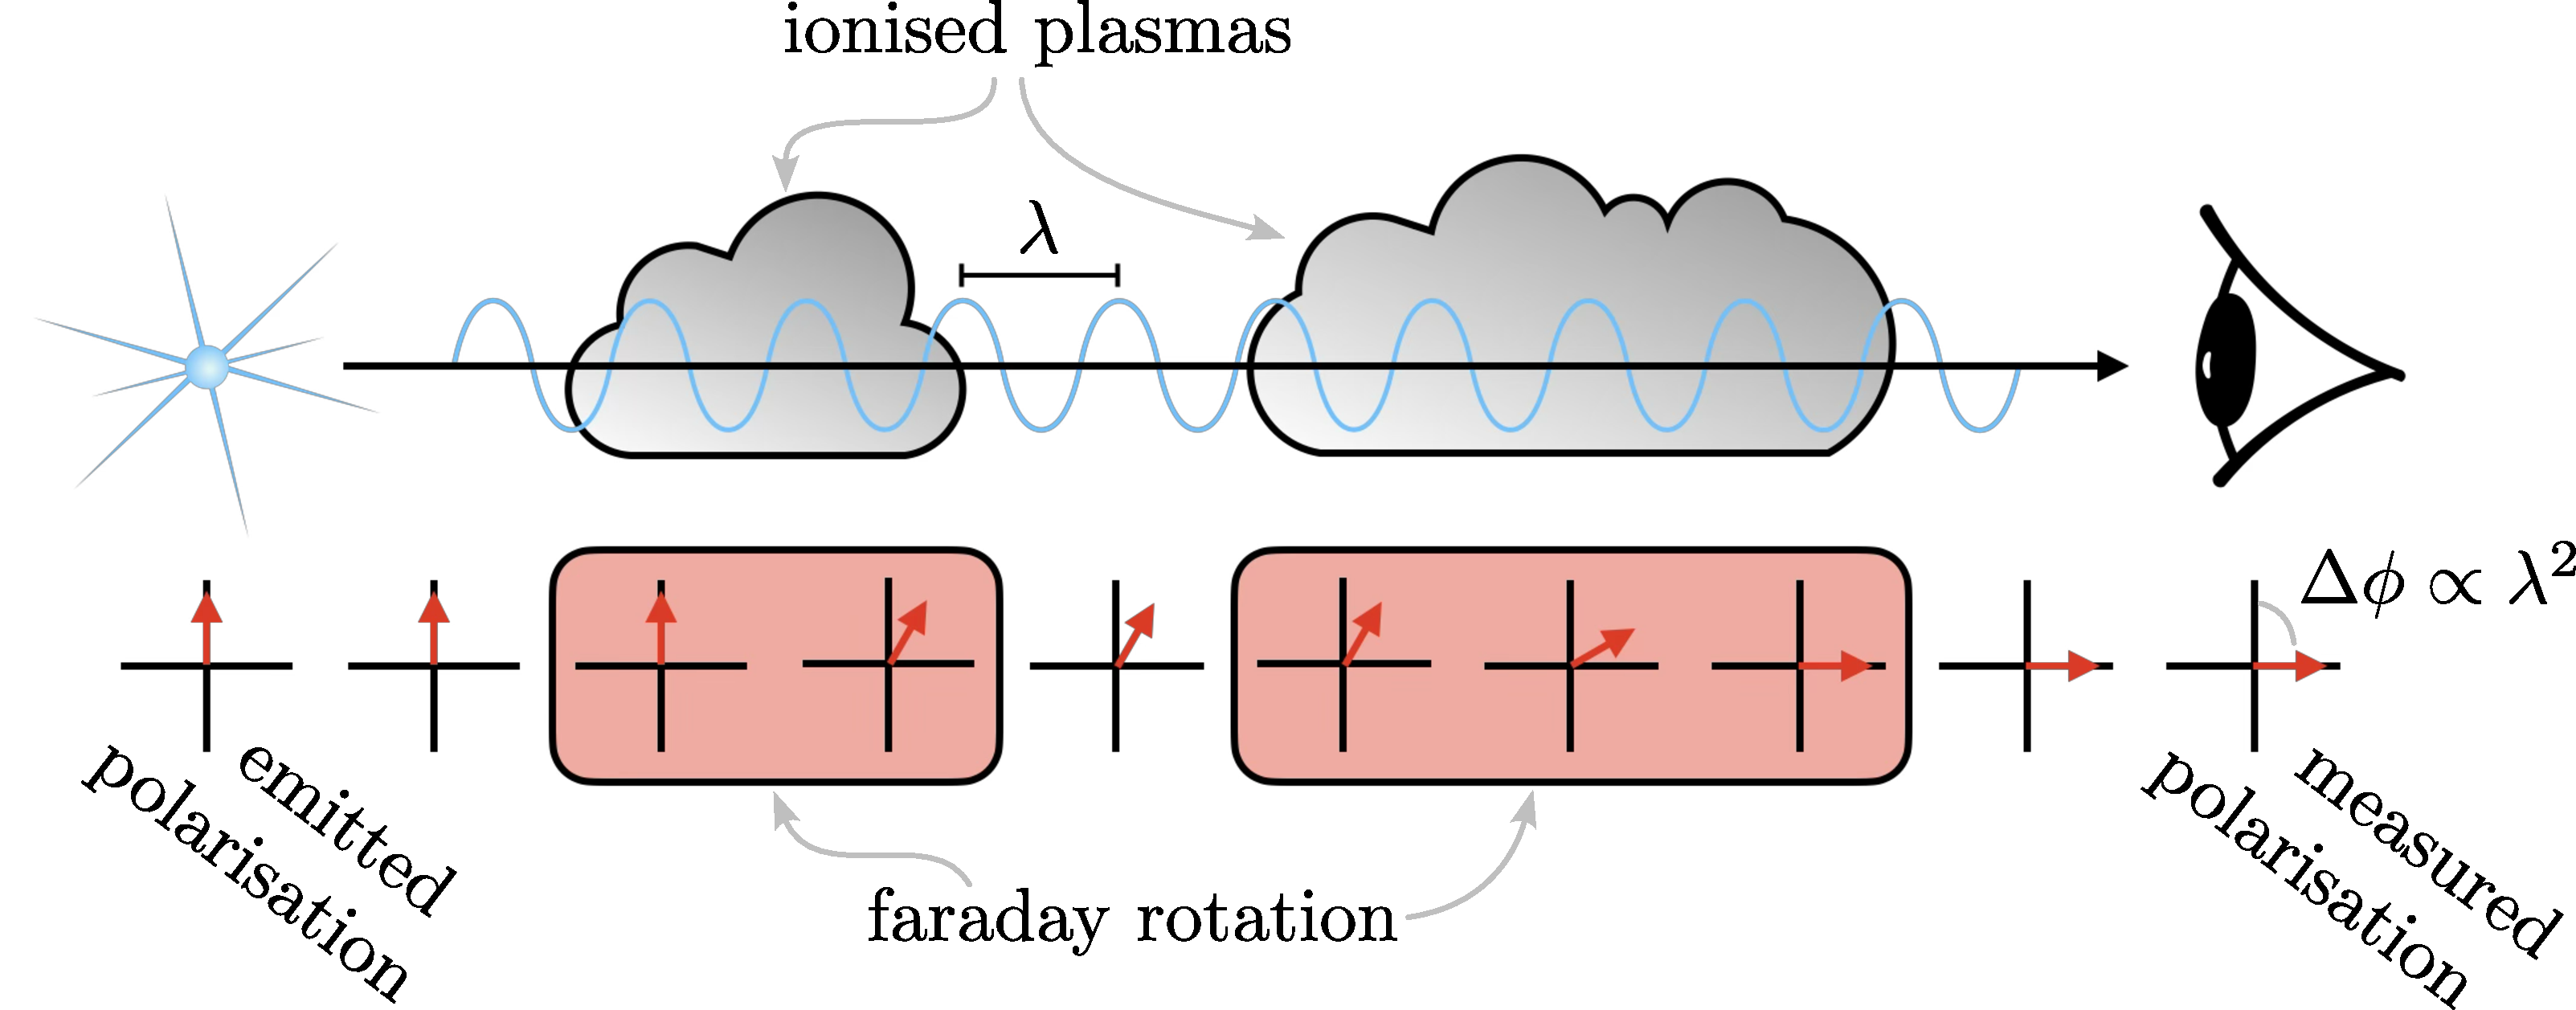
\includegraphics[width=\linewidth]{figures/introduction/faraday.pdf}
    \caption{Schematic of Faraday rotation. Linearly polarised radiation emitted by a background source propagates through regions of ionised plasma, causing the polarisation angle, $\phi$, to rotate. The accumulated rotation depends on wavelength as $\Delta\phi \propto \lambda^{2}$, with the rate of rotation quantified by the rotation measure (see \autoref{eqn:how-we-see:RM}).}
    \label{fig:faraday}
\end{figure}

In realistic astrophysical plasmas, however, $b_\parallel$ can reverse many times along the line of sight, so positive and negative contributions often lead to integrated $\mathrm{RM}$ that nearly cancel \citep{haverkorn2014magnetic}. As a consequence, in practice, $\mathrm{RM}$ primarily traces the net, large-scale component of $b_\parallel$, while small-scale structures are imprinted as fluctuations in $\mathrm{RM}$ across neighbouring sightlines, and as depolarisation of the polarised emission. Interpreting $\mathrm{RM}$ in terms of a field strength therefore benefits from independent constraints on $n_\mathrm{th}$, and from combining Faraday rotation with synchrotron intensity and polarisation to jointly constrain $b_\parallel$ and $b_\perp$.

\subsubsection{Dust Polarisation}
\label{sec:how-we-see:polarisation}

\begin{figure}
    \centering
    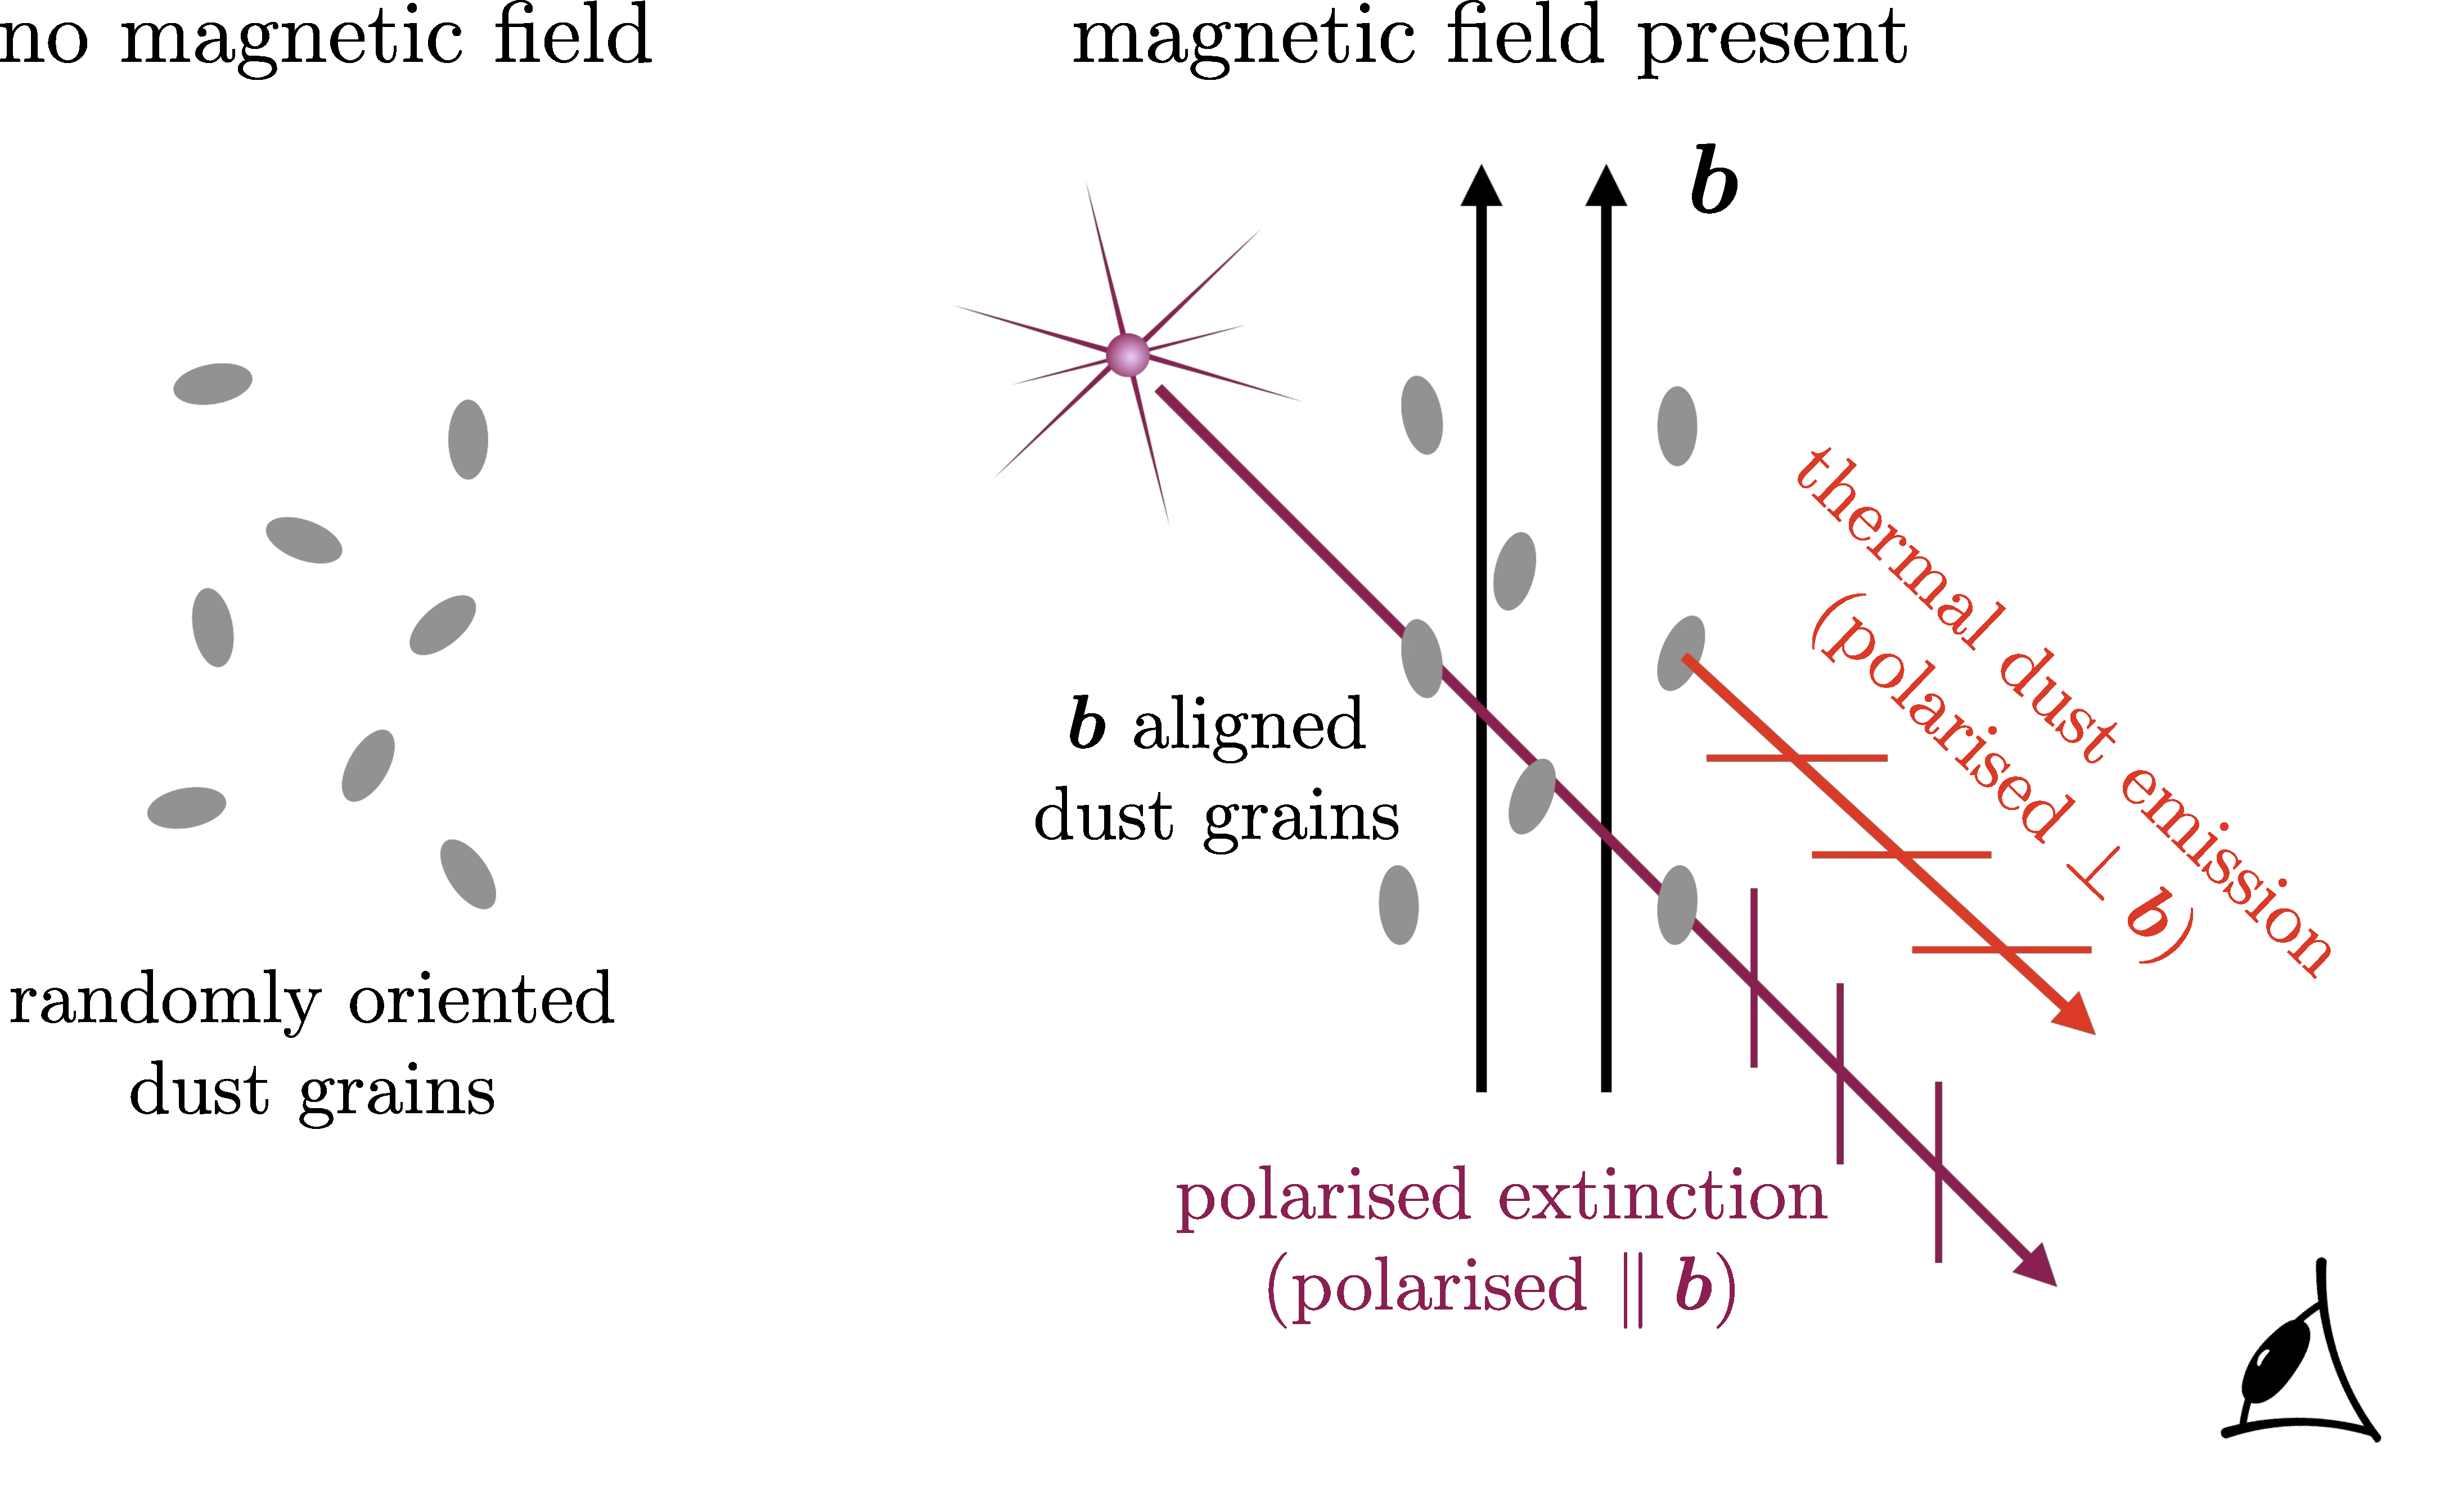
\includegraphics[width=\linewidth]{figures/introduction/dust.pdf}
    \caption{Schematic of dust polarisation, adapted from a lecture by Jennifer Schober. In the absence of a magnetic field (left), dust grains are randomly oriented and produce little net linear polarisation. When a magnetic field is present (right), elongated grains become preferentially aligned with the local field direction, $\mVector{b}$, so that both polarised extinction of background starlight (with polarisation aligned parallel to $\mVector{b}$) and polarised thermal emission (with polarisation aligned perpendicular to $\mVector{b}$) can be used to trace magnetic-field orientation.}
    \label{fig:dust}
\end{figure}

The final probe we will discuss is dust polarisation, which, like synchrotron polarimetry, traces the plane-of-sky magnetic field component, $b_\perp$, through measurements of linear polarisation. At far-infrared and sub-millimeter wavelengths\footnote{
    Faraday rotation is typically negligible at these wavelengths. To see why, consider \autoref{eqn:how-we-see:RM} for a typical diffuse ISM sightline, where $n_\mathrm{th}\sim 0.03~\mathrm{cm^{-3}}$, $b_\parallel\sim 3~\mu\mathrm{G}$, and $L\sim 1~\mathrm{kpc}$. With this, an order-of-magnitude analysis gives $\mathrm{RM}\sim 10^2~\mathrm{rad\,m^{-2}}$. Since the amount of rotation scales as $\lambda^2$, an order-unity rotation requires $\lambda \gtrsim 10^{-1}~\mathrm{m}$, and therefore, at wavelengths associated with dust polarisation, namely $\lambda \lesssim 10^{-3}~\mathrm{m}$, rotation is suppressed; for the same sightline, the rotation at $\lambda\lesssim 10^{-3}~\mathrm{m}$ is smaller than at $\lambda\sim 10^{-1}~\mathrm{m}$ by a factor $\left(10^{-3}/10^{-1}\right)^2 \sim 10^{-4}$, so dust polarisation can usually be interpreted without an $\mathrm{RM}$ correction.
    \label{fnote:faraday}
}, these polarisation measurements are dominated by thermal emission from interstellar dust grains, whereas, at optical and near-infrared wavelengths, they are dominated by the polarised extinction of background starlight by dust. In both regimes, a preferred polarisation emerges because interstellar grains are charged and typically elongated rather than spherically symmetric, which leads to them becoming preferentially aligned with the local magnetic field \citep{andersson2015interstellar}. This alignment makes their absorption and emission anisotropic, producing linearly polarised radiation whose orientation traces the ordered component of $b_\perp$ in the dust-bearing gas (see \autoref{fig:dust}).

Because dust is abundant in the cold and warm phases of the interstellar medium, particularly in filaments and star-forming clouds, dust polarisation is often the most effective cartographer of $b_\perp$ in these environments \citep{collaboration2015planck}. However, dust polarisation on its own only provides a very limited direct constraint on field strength, since the polarisation fraction does not only depend on the field geometry, but also on dust grain properties, alignment efficiency, and line-of-sight averaging. Its primary utility is therefore in constraining the orientation and coherence of $b_\perp$ in dense, dusty environments where synchrotron emission may be weak and Faraday rotation may be hard to interpret.

The \textit{structure} of polarisation maps can nevertheless be used to obtain an estimate of $b_\perp$, where a popular approach is the Davis-Chandrasekhar-Fermi method \citep{davis1951polarization, chandrasekhar1953magnetic}, in which turbulent motions are assumed to perturb the plane-of-sky field, producing a dispersion in polarisation angles, $\sigma_\phi$, whose magnitude reflects the ratio of turbulent to magnetic restoring stresses. Combining $\sigma_\phi$ with an estimate of the gas mass density, $\rho$, and a one-dimensional velocity dispersion, $\sigma_u$, inferred from line widths yields an order-of-magnitude estimate,
\begin{align}
    b_\perp
        \sim Q \, \sqrt{4\pi\rho} \, \frac{\sigma_u}{\sigma_\phi}
    ,
\end{align}
where $Q$ is an order-unity calibration factor that absorbs geometric and line-of-sight effects \citep[\eg][]{ostriker2001density}.

\subsection{A (Brief) Excursion Through Astrophysical Plasmas}
\label{sec:what-we-see}

Zeeman splitting has been successfully applied to star-forming, dense molecular clouds, where measurements indicate $b \sim 10-100 \,\mu\mathrm{G}$ in regions undergoing active collapse and feedback (\eg \citealt{sarma2013very}; see also, \eg \citealt{pattle2022magnetic} for a thorough review). Independent dust polarisation and Faraday-based observations are consistent with these estimates, and indicate that the orientation of $b$ remains ordered over entire clouds, at least on scales of $\sim 10 \,\mathrm{pc}$ \citep{collaboration2015planck, fissel2016balloon, tahani2018helical}. Moreover, dust polarisation measurements at far-infrared wavelengths ($\lambda \sim 50-200 \,\mu\mathrm{m}$) extend this picture to denser regions of the Milky Way, revealing similarly ordered magnetic structures in dense, dust-obscured regions of active star formation \citep{lopez2020sofia}. These different probes and surveys point to a common conclusion for magnetic fields in the Milky Way's dense ISM and star-forming clouds: magnetic energy densities fluctuate about equipartition with kinetic and gravitational energy densities. However, one needs to be careful interpreting these measurements directly, since numerical simulations have shown that projection effects and intermittency can complicate the mapping between observed and intrinsic field properties \citep{camacho2023kinetic, hu2023sub, seta2025magnetic}.

Beyond the Milky Way, nearby spiral galaxies provide some of the clearest evidence for galactic magnetic fields. In the grand-design spiral galaxy M51, for example, synchrotron polarisation and rotation measure observations at $6 \,\mathrm{cm}$ reveal a magnetic field organised on $\sim \mathrm{kpc}$ scales, closely tracing the spiral arms of the disc \citep{fletcher2011magnetic}. In contrast, dust polarisation measurements at $154 \,\mu\mathrm{m}$ reveal a field that varies on $\sim 10 \,\mathrm{pc}$ scales across regions of dense molecular ISM \citep{borlaff2021extragalactic}. These measurements (see \autoref{fig:m51}) probe different phases of the ISM, with dust polarisation tracing cold, dense gas that is sensitive to the plane-of-sky orientation of $b$, while synchrotron emission and Faraday rotation sample diffuse magnetised plasma distributed across the disc. The coexistence of these signatures suggests that the galactic magnetic field carries a large-scale component organised across the disc, alongside a component that varies across the turbulent, star-forming ISM. Similar dust polarisation observations with ALMA show that this is not unique to M51, and is instead a common feature of present-day spiral galaxies \citep[\eg][]{belfiori2025dust, de2025grand}.

\begin{figure}
    \centering
    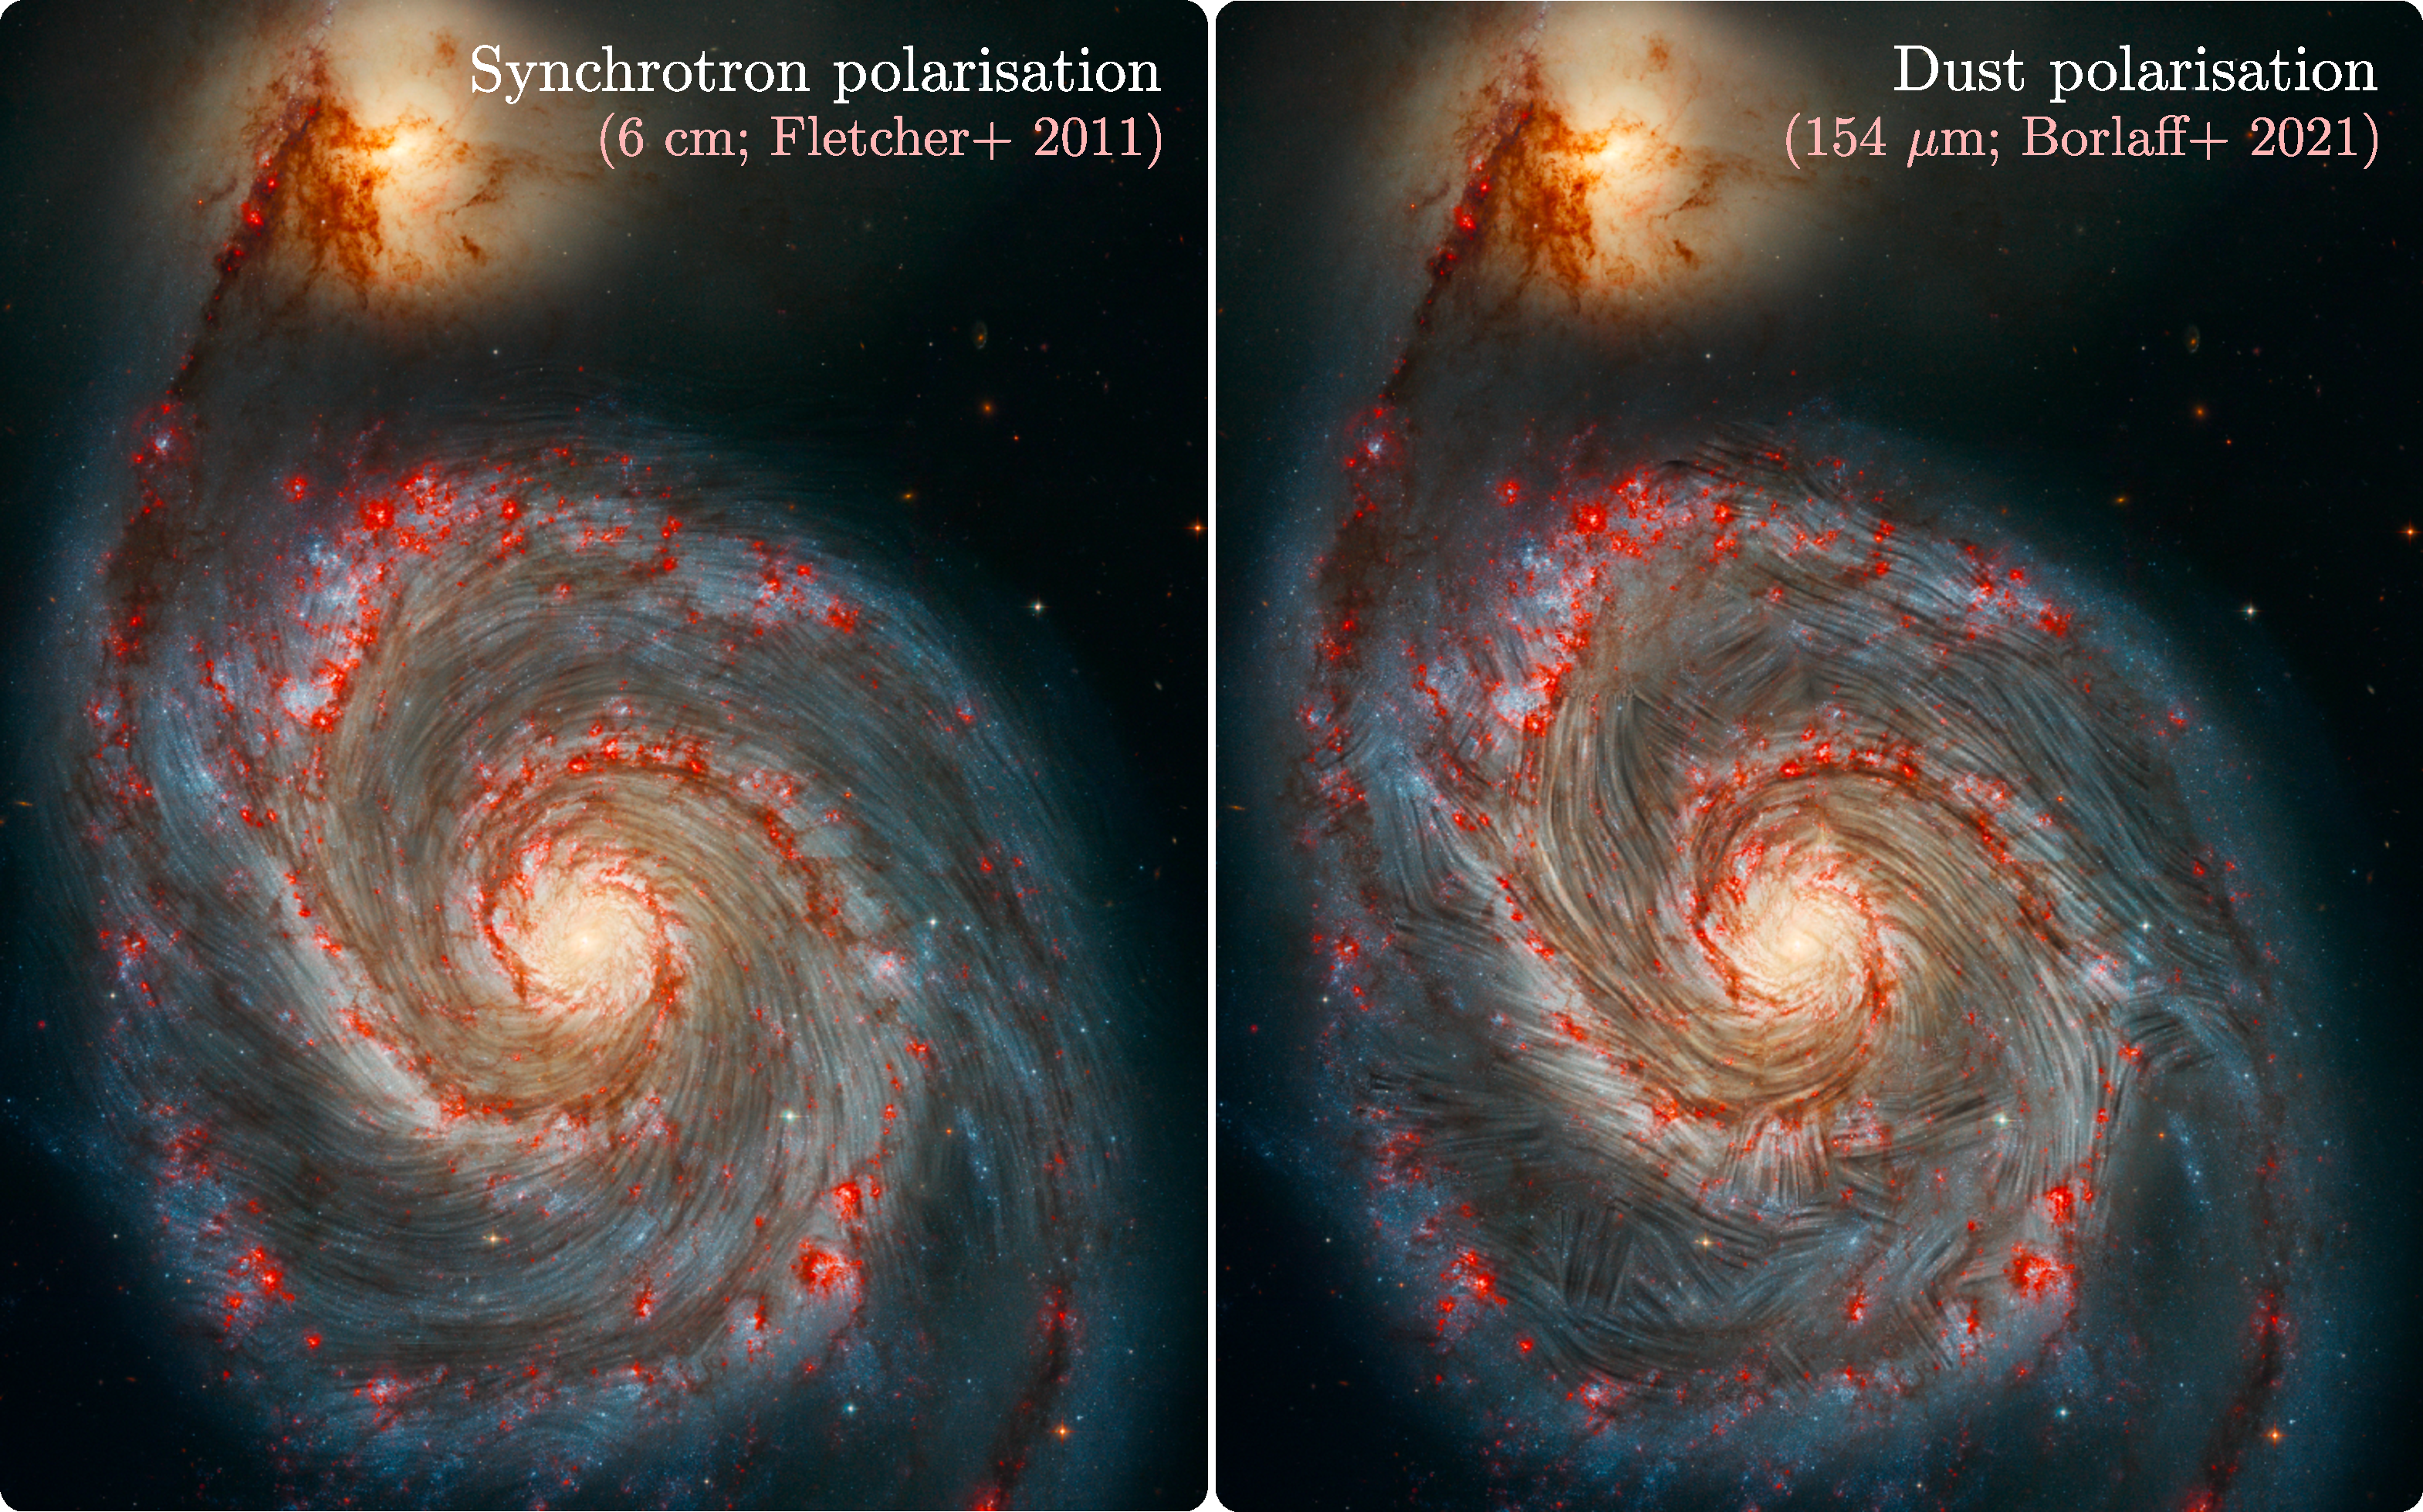
\includegraphics[width=\linewidth]{figures/introduction/M51.pdf}
    \caption{Plane-of-sky magnetic-field orientation in M51 inferred from polarised emission tracing different phases of the interstellar medium. In the left panel, synchrotron polarisation measured at $6\,\mathrm{cm}$ probes the ordered component of the plane-of-sky field, $b_\perp$, in diffuse magnetised plasma \citep{fletcher2011magnetic}; in the right panel, dust polarisation at $154\,\mu\mathrm{m}$ samples colder, denser gas \citep{borlaff2021extragalactic}. In both cases, the polarisation angle constrains the orientation of $b_\perp$ (with only the synchrotron angle susceptible to Faraday rotation along the line of sight; see \autoref{fnote:faraday}).}
    \label{fig:m51}
\end{figure}

Perhaps the most surprising observational result, which, as we discuss below, sits at odds with the current picture of magnetogenesis, is that coherent magnetic fields already appear to be present on $\sim\mathrm{kpc}$ scales in ``young'' galaxies. Rotation-measure studies at $z \sim 1$ indicate ordered line-of-sight field components comparable to those in nearby systems \citep{bernet2008strong, sur2018faraday}. More recently, ALMA detections of polarised dust emission have extended this picture to earlier epochs, revealing ordered plane-of-sky magnetic structures at $z \approx 2.6$ and $z \approx 5.6$ on scales of several $\mathrm{kpc}$ \citep{geach2023polarized, chen2024kiloparsec}. This is particularly surprising, because these ordered fields are usually associated with mechanisms that rely on sustained coherent rotation to organise magnetic structure on galactic scales. These galaxies, however, are placed at epochs where rotationally supported discs are generally not expected to have fully formed (\citealt{geach2023polarized} estimate a dynamo number $\mathcal{D} \approx 3$; see \S\ref{sec:evolve:lsd}). The presence of coherent magnetic fields at such early times therefore poses a significant challenge, and motivates a closer exploration of the circumstances and conditions under which large-scale magnetic structures could be generated in young systems.


\section{Modelling Magnetised Flows}
\label{sec:modelling}

In this chapter we introduce the theoretical framework used to describe the dynamics of magnetised astrophysical flows. Our starting point is a macroscopic fluid description, which is appropriate on the length and timescales relevant for galaxy evolution, where the collective behaviour of large numbers of particles dominates over individual kinetic effects. Since these particles are charged, this naturally leads to the magnetohydrodynamic (MHD) framework, which couples fluid dynamics to electromagnetic fields and provides a self-consistent description of conducting plasmas; these equations form the foundation for the remainder of this thesis.

We begin by introducing the fluid framework and its governing conservation laws (\S\ref{sec:modelling:fluid}), before extending this description to magnetised matter in the MHD framework (\S\ref{sec:modelling:mhd}). We then discuss how magnetic fields can be generated from initially unmagnetised conditions (\S\ref{sec:modelling:magnetogenesis}), and conclude by outlining the principal modes through which magnetic fields subsequently evolve and are maintained in astrophysical systems (\S\ref{sec:evolve}).

\subsection{The Fluid Framework}
\label{sec:modelling:fluid}

Our Universe is made up of many, many particles, each of which is governed, at its most fundamental level, by quantum physics. However, on the astrophysical scales relevant for galaxy dynamics, quantum wave effects are negligible, so particle motion can be described classically, with trajectories determined by Newton's laws of motion. On these scales, tracking trajectories for each particle quickly becomes impractical, since the number of particles in almost all astrophysical systems is enormous. It is instead more useful to adopt a statistical description of particle populations, whereby the collective properties of particles are described through a distribution function $\phi(\mVector{x}, \mVector{v}, t)$, which gives the number density of particles in phase space $(\mVector{x}, \mVector{v})$, where $\mVector{x}$ is the particle's real-space position, $\mVector{v}$ is its velocity, and $t$ is time. At fixed $\mVector{x}$ and $t$, integrating $\phi$ over all velocities gives the local number density,
\begin{align}
    n(\mVector{x}, t)
        \equiv \int \phi(\mVector{x}, \mVector{v}, t)  \mdd^3v .
\end{align}
From this, we can immediately define macroscopic fields describing the fluid of interest through velocity moments of $\phi$. In particular, the fluid density, fluid velocity, and specific (\ie per unit mass) total energy are defined as
\begin{align}
    \rho(\mVector{x}, t)
        &\equiv m \int \phi(\mVector{x}, \mVector{v}, t)  \mdd^3v
        , \\
    \mVector{u}(\mVector{x}, t)
        &\equiv \frac{m}{\rho(\mVector{x}, t)} \int \mVector{v} \phi(\mVector{x}, \mVector{v}, t)  \mdd^3v
        , \\
    \psi^{*}_\mathrm{tot}(\mVector{x}, t)
        &\equiv \frac{m}{2\rho(\mVector{x}, t)}\int \mVector{v}^{ 2} \phi(\mVector{x}, \mVector{v}, t)  \mdd^3v
        ,
\end{align}
with $m$ the particle mass. From this, we can also define other useful quantities, like the specific kinetic energy $\psi^{*}_\mathrm{kin} = u^2 / 2$, and the specific internal energy $\psi^{*}_\mathrm{int} = \psi^{*}_\mathrm{tot} - \psi^{*}_\mathrm{kin}$.

To obtain evolution equations for these macroscopic fields, we require an evolution equation for $\phi$ itself. An intuitive foundation is to realise that conservation of particles in phase space implies a continuity equation of the form
\begin{align}
    \mppFrac{\phi}{t}
        + \nabla_{\mVector{x}} \cdot \rbrac{\mVector{v} \phi}
        + \nabla_{\mVector{v}} \cdot \rbrac{\mppFrac{\mVector{v}}{t} \phi}
        = g(\phi)
        ,  \label{eqn:boltzmann}
\end{align}
where $\mdd_t \mVector{v}$ is the acceleration due to long-range (body) forces, and $g(\phi)$ is a nonlinear operator that captures the net effect of short-range interactions between particles, which, in neutral fluids, are limited to collisions. In collisionless flow regimes (often relevant for diffuse galactic halos and cosmic voids), $g(\phi) \approx 0$ (\autoref{eqn:boltzmann} reduces to the Vlasov equation), but in dense, collisional flow regimes (relevant for the dense interstellar medium and galactic discs), collisions are frequent and drive $\phi$ toward local equilibrium.

Now, notice that the macroscopic conservation laws do not require $g(\phi)$ to be explicitly stated. This is because taking velocity moments of \autoref{eqn:boltzmann} yields conservative evolution equations for mass, momentum, and energy, in which $g(\phi)$ drops out. Ultimately, this occurs because collisions conserve the number of particles, their momentum, and energy. To obtain a closed fluid system we need to relate the higher moments to the evolved fields through a closure; in the ideal-fluid (Euler) limit (where explicit heating and cooling terms are negligible) this enters through an equation of state $p(\rho, \psi^{*}_\mathrm{int})$, which leads to the evolution equations
\begin{align}
    \mppFrac{\rho}{t}
        + \nabla \cdot (\rho \mVector{u})
        &= 0
        , & \mbox{(mass)} \label{eqn:fluid:mass} \\
    \mppFrac{(\rho \mVector{u})}{t}
        + \nabla \cdot \rbrac{
            \rho (\mVector{u}\otimes\mVector{u})
            + p \mTensor{I}
            - \mTensor{V}
        }
        &= \rho \mVector{f}
        , & \mbox{(momentum)} \label{eqn:fluid:momentum} \\
    \mppFrac{(\rho \psi^{*}_\mathrm{tot})}{t}
        + \nabla \cdot \rbrac{
            (\rho \psi^{*}_\mathrm{tot} + p) \mVector{u}
            - \mTensor{V} \cdot \mVector{u}
        }
        &= \rho (\mVector{f}\cdot\mVector{u})
        , & \mbox{(total energy)} \label{eqn:fluid:energy}
\end{align}
that describe the conservative evolution of a single-species, electrically neutral fluid under body forces. Here $\mTensor{V}$ is the viscous stress tensor, which captures the anisotropic part of the pressure (momentum-flux) tensor beyond the Euler closure (isotropic pressure; stresses are the same in every direction; the interested reader is encouraged to consult Chapter 4 of \citealt{shu2010physics}), which we take to be Newtonian with a traceless rate-of-strain form,
\begin{align}
    \mTensor{V}
        \equiv \nu \rho \rbrac{
            \nabla\otimes\mVector{u} + (\nabla\otimes\mVector{u})^\mathsf{T}
            - \frac{2}{3}(\nabla\cdot\mVector{u}) \mTensor{I}
        }
    ,
\end{align}
with kinematic viscosity $\nu$.

\subsection{The Magnetohydrodynamic Framework}
\label{sec:modelling:mhd}

MHD is the natural extension of the fluid framework developed in the previous section to conducting, magnetised matter, in which a sea of charges are able to carry currents. Conceptually, it retains a macroscopic description of matter in terms of fields like $\rho$, $\mVector{u}$, and the specific gas energy $\psi^{*}_\mathrm{tot}$ (equivalently the conserved gas energy density $\psi_\mathrm{tot} = \rho \psi^{*}_\mathrm{tot}$), but augments it to account for the accompanying electromagnetic fields through Maxwell's equations,
\begin{align}
    \mDiv{\mVector{e}}
        &= 4\pi \rho_q
        , & \mbox{(Gauss's law)} \label{eqn:maxwell:gauss} \\
    \mDiv{\mVector{b}}
        &= 0
        , & \mbox{(no magnetic monopoles)} \label{eqn:mhd:monopoles} \\
    \mCurl{\mVector{e}}
        &= -\frac{1}{c} \mppFrac{\mVector{b}}{t}
        , & \mbox{(Faraday's law)} \label{eqn:maxwell:faraday} \\
    \mCurl{\mVector{b}}
        &= \frac{4\pi}{c} \mVector{j} - \frac{1}{c} \mppFrac{\mVector{e}}{t}
        , & \mbox{(Amp\'ere--Maxwell law)} \label{eqn:maxwell:ampere}
\end{align}
where $\mVector{e}$ is the electric field, $\rho_q$ is the charge density, $\mVector{b}$ is the magnetic field, $c$ is the speed of light, and $\mVector{j}$ is the current density. Historically, this coupling between electric and magnetic fields traces back to Faraday's discovery of induction in 1831, which showed that changing magnetic fields generate electromotive forces and currents. Maxwell, who was born in the same year as this discovery, synthesised these ideas into the local field theory embodied by \autoref{eqn:maxwell:gauss}--\ref{eqn:maxwell:ampere} in 1865. However, it was not until Alfv\'en's work in 1942 that it was truly appreciated that this field theory has direct consequences for the dilute, conducting plasmas in galaxies.

Alfv\'en's key realisation was that, although astrophysical plasmas are often extremely dilute, they are also typically more than sufficiently ionised to be efficient conductors. This means they can carry currents ($\mVector{j}$ need not vanish) even though the net charge remains small ($\mAve{\rho_q}_\mVolume \approx 0$) on macroscopic scales. In these regimes, flows are also non-relativistic ($u \ll c$) and quasi-static, so the displacement current term $\mpp_t \mVector{e} / c$ in \autoref{eqn:maxwell:ampere} is negligible and Amp\`ere's law reduces to
\begin{align}
    \mCurl{\mVector{b}}
        = \frac{4\pi}{c} \mVector{j}
        . \label{eqn:mhd-steps:ampere_reduced}
\end{align}
With this, Faraday's law (\autoref{eqn:maxwell:faraday}) can be worked towards an evolution equation for $\mVector{b}$, by using Ohm's law to relate the electric field to the bulk motion in a conducting plasma,
\begin{align}
    \mVector{e}
        = \frac{1}{\sigma} \mVector{j} - \frac{1}{c} \mVector{u}\times\mVector{b}
        ,
    \label{eqn:mhd-steps:ohm}
\end{align}
where $\sigma$ is the electrical conductivity; this lab-frame form of Ohm's law follows from first writing Ohm's law in the local fluid rest frame, and then transforming it into the lab frame (and making use of $u \ll c$). Substituting \autoref{eqn:mhd-steps:ampere_reduced} and \autoref{eqn:mhd-steps:ohm} into \autoref{eqn:maxwell:faraday} yields
\begin{align}
    \mppFrac{\mVector{b}}{t}
        % &= -c \mCurl{\mVector{e}}
        %     \nonumber \\
        % &= \mCurl{(\mVector{u}\times\mVector{b})}
        %     - \eta \mCurl{\mCurl{\mVector{b}}}
        %     \nonumber \\
        &= \mCurl{(\mVector{u}\times\mVector{b})}
            + \mCurl{(\eta \mCurl{\mVector{b}})}
            , \label{eqn:mhd-steps:induction}
\end{align}
where $\eta = c^2/(4\pi\sigma)$ is the magnetic diffusivity, and $\mDiv{\mVector{b}} = 0$ was used.

Finally, once the fluid carries currents, magnetic fields influence the flow of gas through forces that act on those currents. This is reflected by Lorentz force terms in both \autoref{eqn:fluid:momentum} and \autoref{eqn:fluid:energy}. Taking these updated evolution equations together with the induction equation, \autoref{eqn:mhd-steps:induction}, yields the compressible, visco-resistive MHD equations in conservative form,
\begin{align}
    \mppFrac{\rho}{t} + \nabla \cdot (\rho \mVector{u})
        &= 0
        , \label{eqn:mhd:mass} \\
    \mppFrac{(\rho \mVector{u})}{t}
        + \nabla \cdot \rbrac{
            \rho \mVector{u}\otimes\mVector{u}
            + \rbrac{p + \psi_\mathrm{mag}} \mTensor{I}
            - \frac{\mVector{b}\otimes\mVector{b}}{4\pi}
            - \mTensor{V}
        }
        &= \rho \mVector{f}
        , \label{eqn:mhd:momentum} \\
    \mppFrac{\psi_\mathrm{tot}}{t}
        + \nabla \cdot \left(
            \rbrac{\psi_\mathrm{tot} + p + \psi_\mathrm{mag}} \mVector{u}
            - \frac{(\mVector{u}\cdot\mVector{b})\mVector{b}}{4\pi}
            - \mTensor{V}\cdot\mVector{u}
            \right.\nonumber\nquad[1]&\\
            \left.
            - \frac{\eta}{4\pi} \mVector{b}\times(\mCurl{\mVector{b}})
        \right)
        &= \rho \mVector{f} \cdot \mVector{u}
        , \label{eqn:mhd:energy} \\
    \mppFrac{\mVector{b}}{t}
        + \nabla \cdot \rbrac{
            \mVector{u}\otimes\mVector{b} - \mVector{b}\otimes\mVector{u}
        }
        &= -\mCurl{(\eta \mCurl{\mVector{b}})}
        , \label{eqn:mhd:induction}
\end{align}
where the total energy density,
\begin{align}
    \psi_\mathrm{tot}
        \equiv \rho\rbrac{
                \psi^{*}_\mathrm{int}
                + \psi^{*}_\mathrm{kin}
            }
            + \psi_\mathrm{mag}
    ,
\end{align}
has been updated to include the magnetic energy reservoir $\psi_\mathrm{mag} \equiv b^2 / (8\pi)$.

To close the system, we require an equation of state $p(\rho, \psi^{*}_\mathrm{int})$, so, here, and in the remainder of this thesis, we will adopt an isothermal closure $p = c_s^2 \rho$ (where $c_s$ is the sound speed), and therefore the thermal state becomes directly set by $\rho$, and $\psi^{*}_\mathrm{int}$ is no longer an independent quantity. In this configuration, \autoref{eqn:mhd:energy} does not need to be considered explicitly, with the dynamics fully determined by \autoref{eqn:mhd:mass}-\ref{eqn:mhd:induction}, with \autoref{eqn:mhd:monopoles} remaining an important supplementary constraint.

\subsection{Flavours of Magnetogenesis}
\label{sec:modelling:magnetogenesis}

While the visco-resistive MHD framework developed in \autoref{eqn:mhd:mass}--\ref{eqn:mhd:induction} can successfully describe the evolution of magnetised flows (see \S\ref{sec:evolve}), it implicitly assumes that a magnetic field already exists. However, if $\psi_\mathrm{mag} = 0$ initially, then \autoref{eqn:mhd:induction} does not provide a means through which $\psi_\mathrm{mag} \neq 0$ can be generated. This form of the induction equation is appropriate for the present-day Universe, where magnetic fields appear to be ubiquitous, even when weak. However, magnetic fields are not expected to have existed ab initio. This is because, as Amp\`ere's law (\autoref{eqn:mhd-steps:ampere_reduced}) reveals, magnetic fields are inseparable from electric currents and thereby the organised flow of charges. In the standard $\Lambda$CDM model, the early Universe is expected to have been homogeneous and charge-neutral, and therefore to lack large-scale, organised currents. Thus the generation of $\psi_\mathrm{mag} > 0$ must have involved a process capable of generating currents ex nihilo in an initially unmagnetised plasma. A number of plausible mechanisms have been proposed that can achieve this, but here we will focus on the Biermann battery \citep{biermann1950ursprung} as an example, and refer the interested reader to, \eg \citet{widrow2012first} and \citet{subramanian2016origin} for comprehensive reviews of seed mechanisms.

In the context of \autoref{eqn:mhd:induction}, the seeding of $\mVector{b}$ can be traced back to the closure adopted for $\mVector{e}$. For the single-fluid regime, where electron and ion motions are strongly coupled, this closure is provided by Ohm's law\footnote{
    Historically an empirical relation for electrical conductors, but one that naturally extends to the continuum regime.
} (\autoref{eqn:mhd-steps:ohm}), which is appropriate on macroscopic scales. However, electron and ion motions need not remain tightly coupled on sufficiently small scales. This is because ions are much heavier than electrons, and therefore a gas pressure gradient accelerates the two species at (slightly) different rates. The resulting relative drift between these species drives an electric current that introduces extra contributions to $\mVector{e}$, even though the medium remains globally quasi-neutral. These effects lead to a generalised Ohm's law of the form
\begin{align}
    \mVector{e}
        = \overbrace{
                \frac{1}{\sigma} \,\mVector{j}
            }^\text{Ohmic resistivity}
            - \underbrace{
                \frac{1}{c} \,\mVector{u}\times\mVector{b}
            }_\text{induction}
            + \overbrace{
                \frac{1}{q_e n_e c} \,\mVector{j}\times\mVector{b}
            }^\text{Hall effect}
            - \underbrace{
                \frac{1}{q_e n_e} \nabla p_e
            }_\text{electron pressure}
    ,
\end{align}
where $n_e$ and $p_e$ are the electron number density and pressure, respectively. When $\psi_\mathrm{mag} = 0$ initially, the induction and Hall terms vanish identically, since the former is directly proportional to $\mVector{b}$, and the latter to $\mVector{j} \propto \nabla\times\mVector{b}$ through Amp\`ere's law: both depend on a field that does not yet exist. If $\sigma$ is also spatially uniform, the curl of the Ohmic term reduces to an expression in $\mVector{b}$ through the same relation, and so it too vanishes. The electron pressure-gradient term is therefore the only contribution to $\nabla\times\mVector{e}$ that can survive when no field yet exists, which is precisely what allows it to seed $\mVector{b}$ from nothing. Substituting this term into Faraday's law (\autoref{eqn:maxwell:faraday}) gives
\begin{align}
    \mCurl{\rfrac{\nabla p_e}{q_e n_e}}
        = \frac{1}{q_e}\frac{\nabla n_e \times \nabla p_e}{n_e^2}
\end{align}
in \autoref{eqn:mhd:induction}. This is the Biermann battery, and it operates in baroclinic flows where $\nabla n_e$ and $\nabla p_e$ are not aligned. The battery term vanishes identically in barotropic plasmas, where $p_e = p_e(n_e)$ and so $\nabla p_e \parallel \nabla n_e$; efficient seeding therefore requires a process that breaks this alignment, such as the reionisation fronts discussed below.

The Biermann battery is one member of a broader family of mechanisms that generate $\nabla\times\mVector{e} \neq 0$ through some channel other than induction or Hall currents. The Durrive battery \citep{durrive2015intergalactic}, for example, instead sources $\mVector{b}$ through anisotropic radiation pressure imparted by photoionisation fronts, rather than through baroclinic misalignment of $\nabla n_e$ and $\nabla p_e$.

\begin{figure}
    \centering
    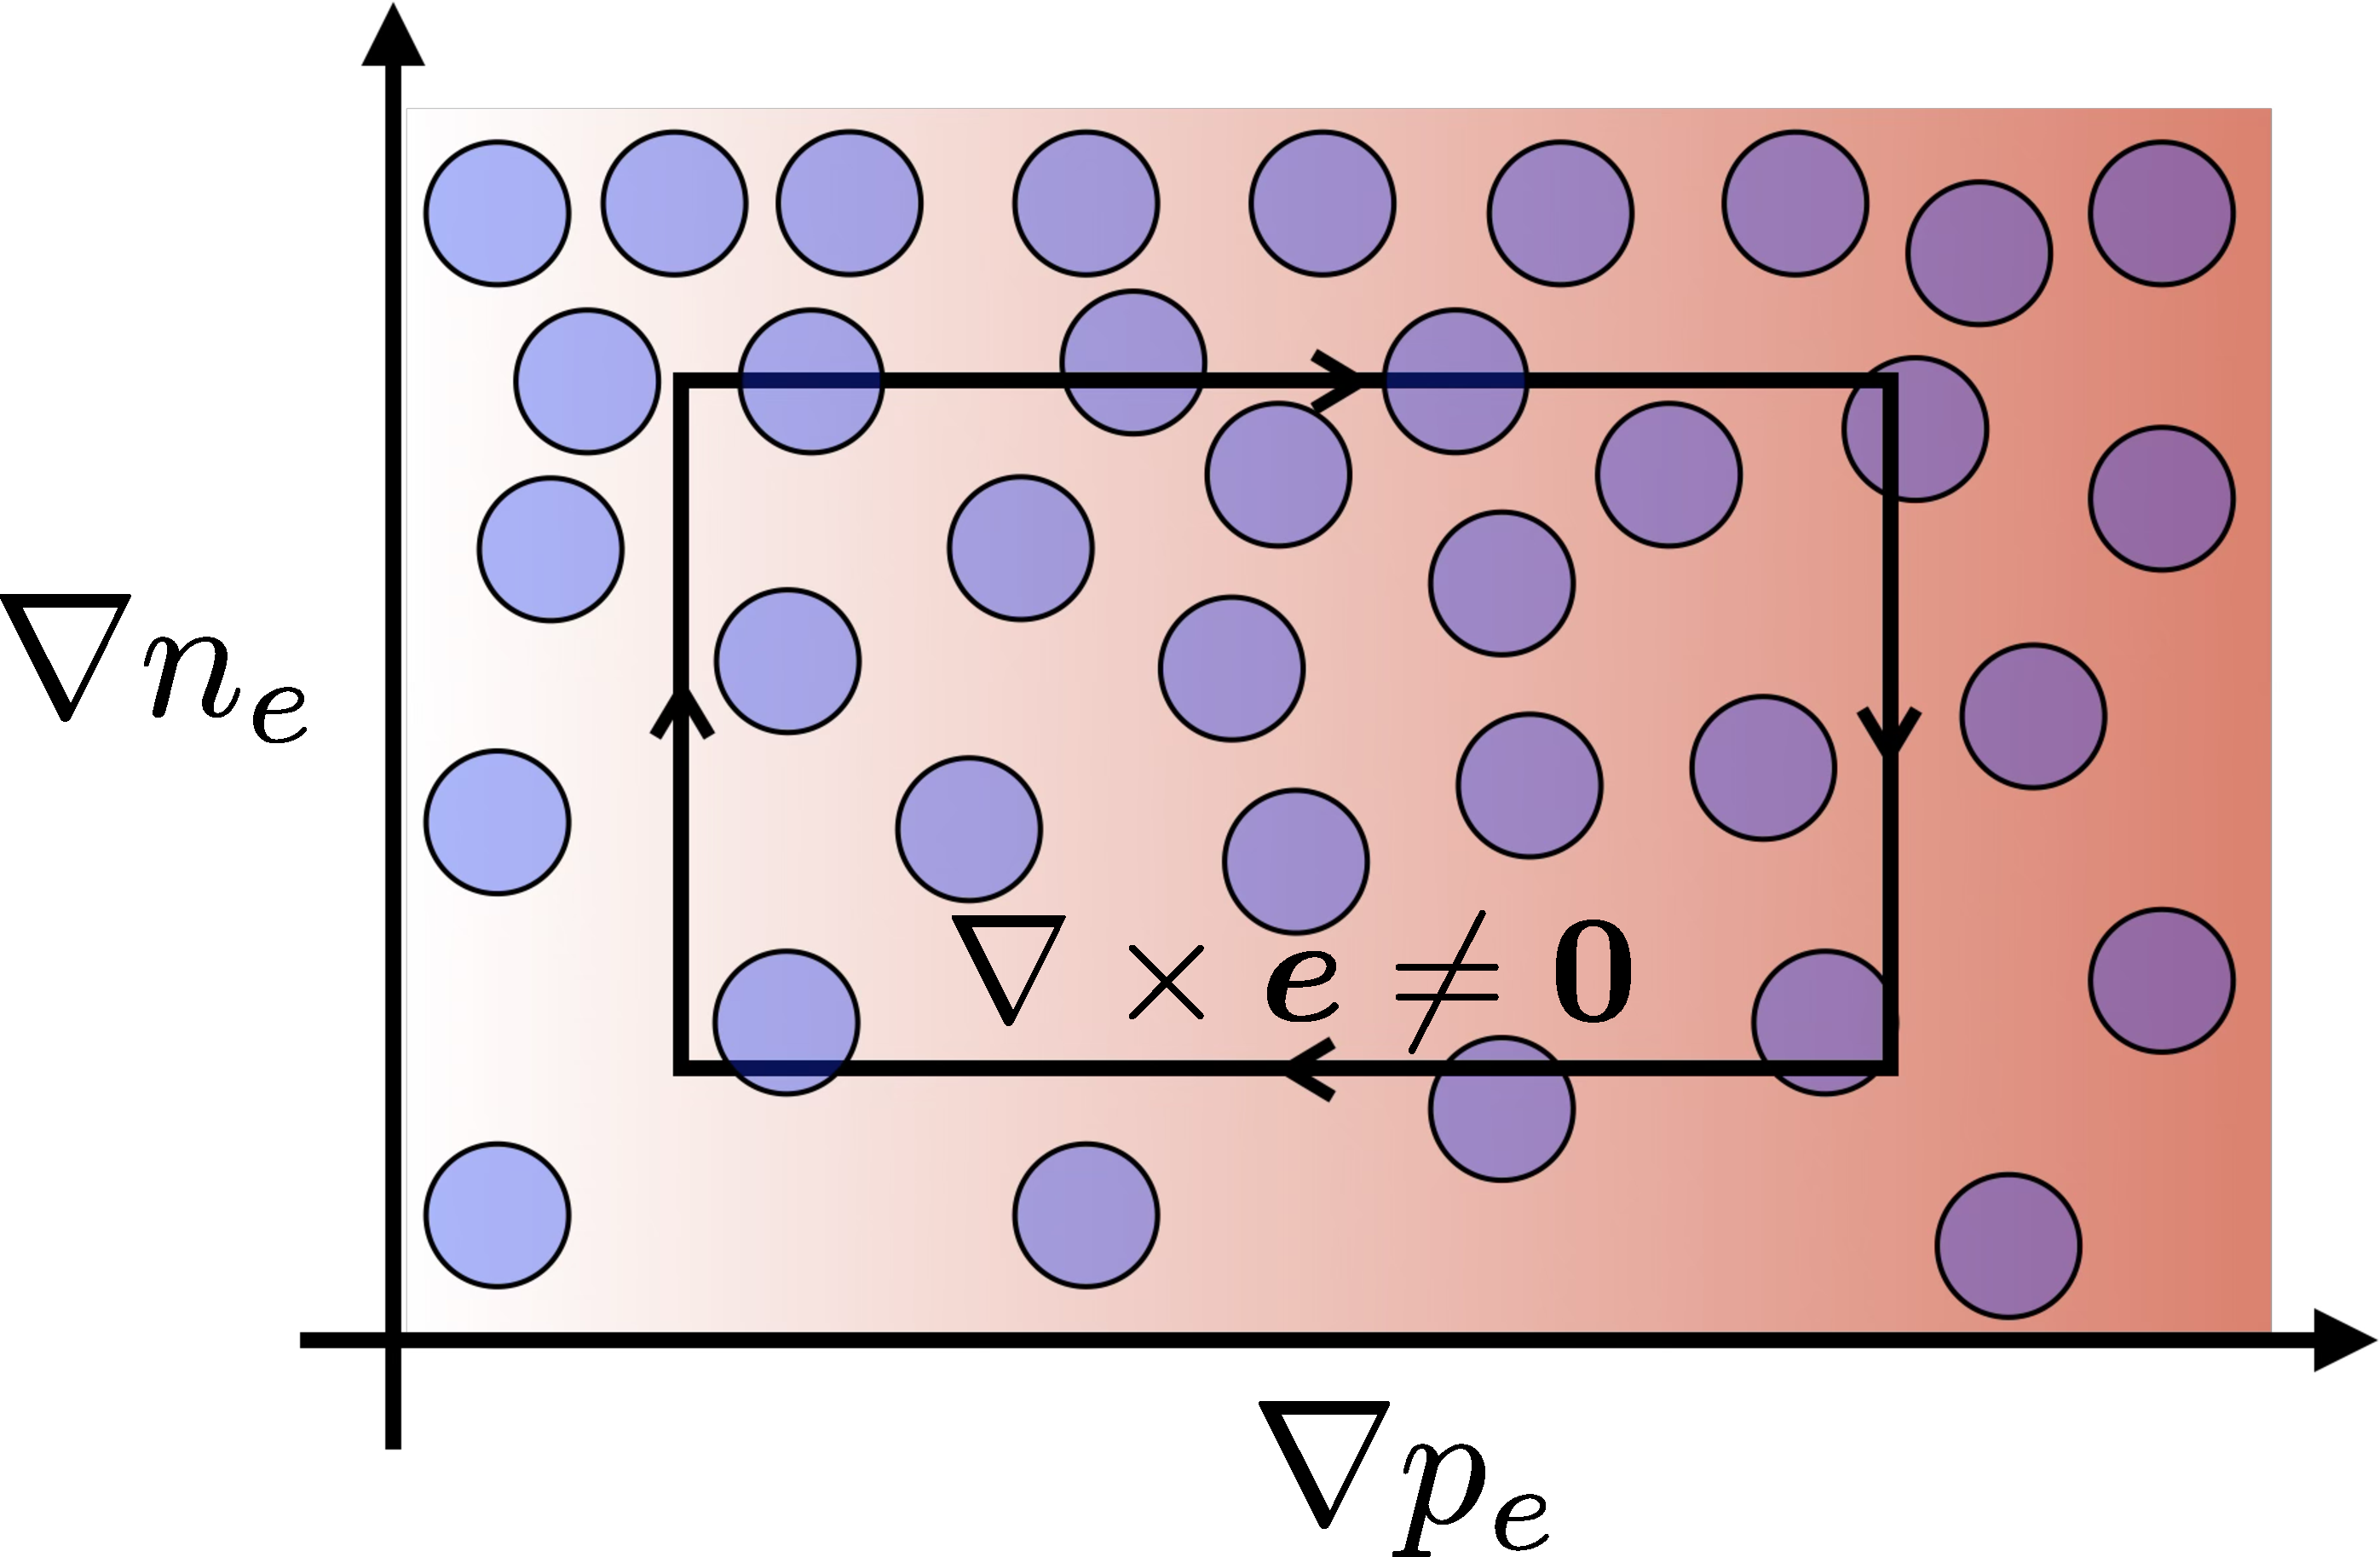
\includegraphics[width=0.65\linewidth]{figures/introduction/biermann.pdf}
    \caption{Schematic of Biermann battery seeding, adapted from a lecture by Jennifer Schober. In a baroclinic plasma, gradients in electron density and electron pressure are not aligned, so $\nabla n_e \times \nabla p_e \neq \mVector{0}$. The electron pressure term in the generalised Ohm's law then produces a non-zero curl of the electric field, $\nabla\times\mVector{e} = (1/q_e)\,(\nabla n_e \times \nabla p_e)/n_e^2$, which yields a non-zero electromotive circulation around a loop. Through Faraday's law, this drives $\partial \mVector{b}/\partial t \neq 0$ and generates a seed magnetic field even when $\mVector{b}=0$ initially.}
    \label{fig:placeholder}
\end{figure}

\citet{gnedin2000generation} was among the first to demonstrate the Biermann battery operating in a cosmological simulation, showing that baroclinic structures naturally form in the reionisation fronts surrounding protogalaxies. They found that this generates volume-filling seed fields of $b \sim 10^{-19} \,\mathrm{G}$, with stronger $b \gtrsim 10^{-18} \,\mathrm{G}$ in actively forming haloes. More recently, \citet{attia2021cosmological} and \citet{garaldi2021magnetogenesis} revisited this problem by solving the coupled radiation-MHD system self-consistently\footnote{
    \citet{gnedin2000generation} followed Biermann seeding in a decoupled, kinematic regime (see its definition in \S\ref{sec:evolve:paths}), evolving $\mVector{b}$ as a passive field. \citet{attia2021cosmological} and \citet{garaldi2021magnetogenesis} instead evolved $\mVector{b}$ self-consistently.
}, confirming that reionisation fronts provide the dominant Biermann seeding channel in cosmological settings. \citet{attia2021cosmological} further showed that the net seed field receives contributions from multiple epochs, including $b \sim 10^{-25} \,\mathrm{G}$ from weak pre-reionisation seeding during linear structure growth, and $b \sim 10^{-18} \,\mathrm{G}$ in hot, shock-heated bubbles driven by stellar feedback around massive galaxies.

Focusing on the subsequent fate of these extremely weak seed fields, \citet{garaldi2021magnetogenesis} showed that the $\mVector{b}$ that ultimately threads galaxies does not retain the structural properties of its seed topology. Instead, $\mVector{b}$ is amplified during galaxy formation by a mixture of collapse-driven compression and chaotic motions that stretch and fold the field (see \S\ref{sec:evolve:paths} for a discussion on evolution channels for galactic magnetic fields), so present-day galactic fields need not resemble their original configuration. \citet{garaldi2021magnetogenesis} further found that even when $\mVector{b}$ is generated through different battery models (including the photoionisation-driven Durrive battery \citep{durrive2015intergalactic}), the properties of $\mVector{b}$ in dense galactic gas converge toward similar states. This insensitivity to the seed mechanism is not universal, however, and the most diffuse environments remain more sensitive to their initial conditions. \citet{mtchedlidze2022evolution} investigated this explicitly by imposing different primordial seed strengths and topologies in cosmological simulations, and then following the field through large-scale structure formation. They showed that the clearest differences persist in the most rarefied regions of the cosmic web, particularly in cosmic voids. Magnetic fields in voids therefore provide one of the clearest observational tests of competing magnetogenesis scenarios.

\subsection{Flavours of Magnetic Evolution}
\label{sec:evolve}

Once $\psi_\mathrm{mag} > 0$ has been seeded, \autoref{eqn:mhd:mass}--\ref{eqn:mhd:monopoles} become sufficient to describe the evolution of magnetised plasmas. These equations admit a wide range of flow regimes, with various force terms playing different roles. It therefore becomes useful to think about the relative importance of these terms, and the kinds of dynamics they can produce. To expose this, we non-dimensionalise the evolution equations by introducing a characteristic length scale $\ell_0$, bulk velocity $u_0$, density $\rho_0,$ and magnetic amplitude $b_0$, which allow us to define dimensionless variables
\begin{align}
    \tilde{t}
        = \frac{u_0}{\ell_0} t
        , \qquad
    \tilde{\mVector{x}}
        = \frac{\mVector{x}}{\ell_0}
        , \qquad
    \tilde{\rho}
        &= \frac{\rho}{\rho_0}
        , \qquad
    \tilde{\mVector{u}}
        = \frac{\mVector{u}}{u_0}
        , \qquad
    \tilde{\mVector{b}}
        = \frac{\mVector{b}}{b_0}
        \\
    \tilde{\nabla}
        = \ell_0 \nabla
        , \qquad &\mbox{and} \qquad
    \tilde{\mTensor{V}}
        = \frac{\ell_0}{\nu \rho_0 u_0} \mTensor{V}
    .
\end{align}
Substituting these into \autoref{eqn:mhd:momentum} and setting $\mVector{f} = \mVector{0}$ (for convenience) yields the dimensionless momentum equation
\begin{align}
    \mppFrac{(\tilde{\rho} \tilde{\mVector{u}})}{\tilde{t}}
        + \tilde{\nabla} \cdot \rbrac{
            \tilde{\rho} (\tilde{\mVector{u}} \otimes \tilde{\mVector{u}})
            + \frac{1}{\mSonicMach^2} \tilde{\rho} \mTensor{I}
            + \frac{1}{\mAlfvenMach^2} \rbrac{
                \frac{\tilde{b}^2}{2} \mTensor{I}
                - \tilde{\mVector{b}} \otimes \tilde{\mVector{b}}
            }
            + \frac{\tilde{\mTensor{V}}}{\mReh}
        }
        = 0
    ,
\end{align}
where
\begin{align}
    \mSonicMach
        \equiv \frac{u_0}{c_s}
        , \qquad
    \mAlfvenMach
        \equiv \frac{\sqrt{4\pi\rho_0} u_0}{b_0}
        , \qquad \mbox{and} \qquad
    \mReh
        \equiv \frac{u_0\ell_0}{\nu}
        \sim \frac{
            \|\nabla\cdot(\rho\,\mVector{u}\otimes\mVector{u})\|
        }{
            \|\nabla\cdot\mTensor{V}\|
        }
    ,
    \label{defn:Reh}
\end{align}
measure the degree of compressibility, the relative importance of inertial to magnetic stresses, and the relative importance of inertial to viscous stresses (see \S\ref{sec:evolve:ssd}), respectively. It is also useful to compare the relative thermal and magnetic pressure reservoirs, which is captured by
\begin{align}
    \beta
        \equiv 2 \rfrac{\mAlfvenMach}{\mSonicMach}^2
    , \label{defn:plasma-beta}
\end{align}
and indicates when flows are magnetically dominated ($\beta \ll 1$), and conversely when they are hydrodynamically dominated ($\beta \gg 1$).

Similarly, when we non-dimensionalise \autoref{eqn:mhd:induction},
\begin{align}
    \mppFrac{\tilde{\mVector{b}}}{\tilde{t}}
        = \tilde{\nabla} \times \rbrac{\tilde{\mVector{u}}\times\tilde{\mVector{b}}}
            + \frac{1}{\mRem}\,\tilde{\nabla}^2 \tilde{\mVector{b}}
        ,
\end{align}
we are introduced to
\begin{align}
    \mRem
        \equiv \frac{u_0\ell_0}{\eta}
        \sim \frac{
                \|\nabla\times(\mVector{u}\times\mVector{b})\|
            }{
                \|\mCurl{(\eta\mCurl{\mVector{b}})}\|
            }
    ,
    \label{defn:Rem}
\end{align}
which measures the relative importance of inductive advection to resistive diffusion (see \S\ref{sec:evolve:decay}).

\begin{figure}
    \centering
    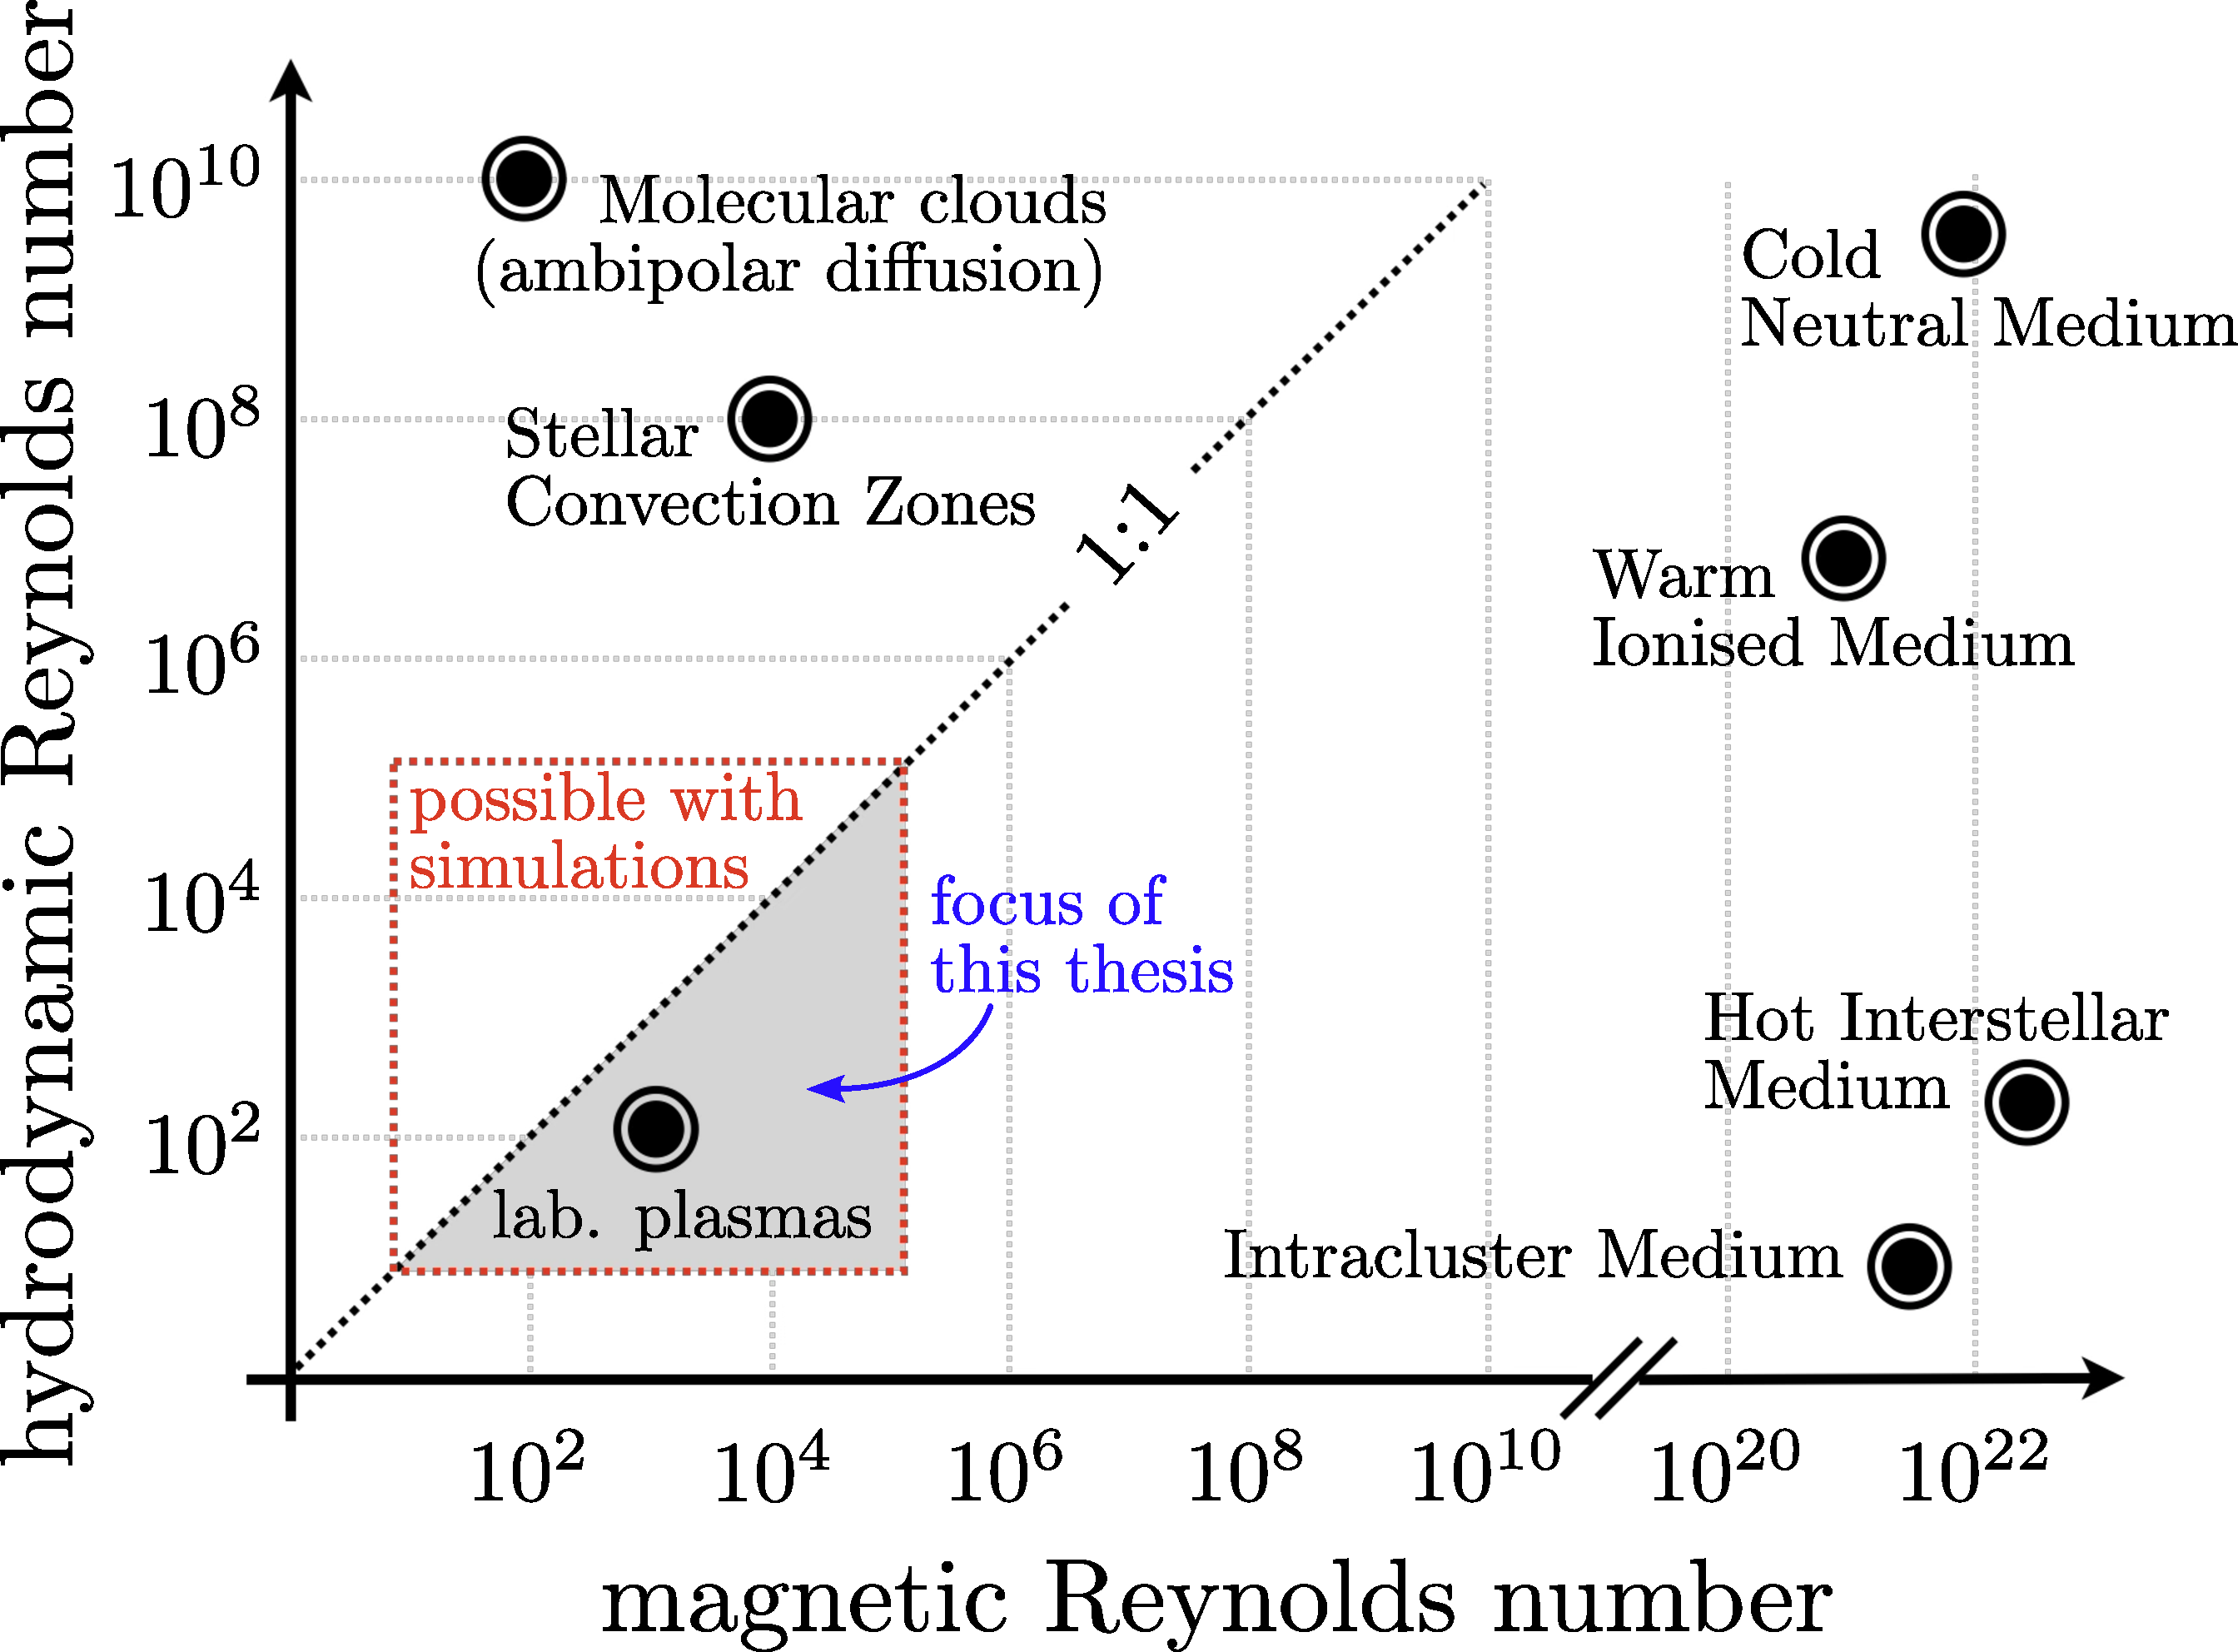
\includegraphics[width=0.8\linewidth]{figures/introduction/regimes.pdf}
    \caption{Order-of-magnitude hydrodynamic (\autoref{defn:Reh}) and magnetic Reynolds numbers (\autoref{defn:Rem}) for a representative selection of astrophysical environments, using parameters compiled from \citet{rincon2019dynamo} and \citet{brandenburg2023galactic}. These two dimensionless numbers are among the key parameters that diagnose the relative importance of different dynamical processes (see also \autoref{defn:plasma-beta}). A diagonal dotted line shows $\mathrm{Pm} = 1$ (see \autoref{defn:Prm}), for which viscous and resistive dissipation take place on comparable scales. Separately, the red box indicates the region of this parameter space that is currently accessible to direct numerical simulations; for the time being, most realistic astrophysical plasmas remain far out-of-reach, but simulations can nevertheless probe the consequences of different dynamical effects. The grey triangle highlights the subset of this accessible space that is the focus of this thesis.}
    \label{fig:plasma-regimes}
\end{figure}

As \citet{rincon2019dynamo} summarises nicely in a schematic much like \autoref{fig:plasma-regimes}, astrophysical plasmas span a vast range of configurations in the parameter space defined by $\mReh$ and $\mRem$, which are often enormous. In these inertial and inductive dominated flow regimes, it is the relative (rather than absolute) magnitudes of these two numbers that becomes relevant, with the magnetic Prandtl number
\begin{align}
    \mPrm
        &= \frac{\mRem}{\mReh}
        \sim \frac{\nu}{\eta}
    , \label{defn:Prm}
\end{align}
providing a convenient measure of the separation between viscous and resistive effects. In this thesis we exclusively focus on the $\mPrm \geq 1$ regime, which is relevant for many diffuse astrophysical plasmas, including the $\mSonicMach \gtrsim 1$, $\mReh \gg 1$ turbulence in the interstellar medium, where galactic magnetic fields are thought to be maintained.

\subsubsection{The Dynamical Roads Along Which Magnetism Walks}
\label{sec:evolve:paths}

One of the key takeaways from our discussion of magnetogenesis in \S\ref{sec:modelling:magnetogenesis} is that, while there are many plausible mechanisms capable of seeding the first magnetic fields, none produced the fields we observe in the present-day Universe (\eg those discussed in \S\ref{sec:what-we-see}) in their present form. For one, seed fields are far weaker than the magnetic fields we infer today. The magnetic fields we see, whether on the scales of molecular clouds in the interstellar medium, or threading galactic discs and halos, must therefore have undergone substantial amplification and reorganisation ever since they were seeded.

For much of this magnetic history, galactic fields are expected to have been dynamically weak compared to the motions of the gas, $\psi_\mathrm{mag} \ll \psi_\mathrm{kin}$. In this limit, Lorentz forces become negligible in \autoref{eqn:mhd:momentum}, so, as far as the momentum budget is concerned, the gas evolves as if it were effectively unmagnetised. To leading order, \autoref{eqn:mhd:momentum} therefore reduces back to its hydrodynamic form,
\begin{align}
    \mppFrac{(\rho \mVector{u})}{t}
        + \nabla \cdot \rbrac{
            \rho \mVector{u}\otimes\mVector{u}
            + p \mTensor{I}
            - \mTensor{V}
        }
        &= \rho \mVector{f}
    .
\end{align}
With this, $\mVector{u}$ evolves independently of $\mVector{b}$, and \autoref{eqn:mhd:induction} becomes linear in $\mVector{b}$. It follows that the instantaneous fractional evolution of magnetic energy density,
\begin{align}
    \mDDFrac{(\ln\psi_\mathrm{mag})}{t}
        = \frac{1}{\psi_\mathrm{mag}} \mDDFrac{\psi_\mathrm{mag}}{t}
        = \frac{2\mVector{b}}{b^2} \cdot \mDDFrac{\mVector{b}}{t}
    ,
\end{align}
does not depend on the magnitude of $\psi_\mathrm{mag}$; here $\mDD / \mDD t \equiv \partial/\partial t + \mVector{u}\cdot\nabla$ is the material derivative. This flow regime is popularly referred to as \textit{kinematic}.

\begin{figure}
    \centering
    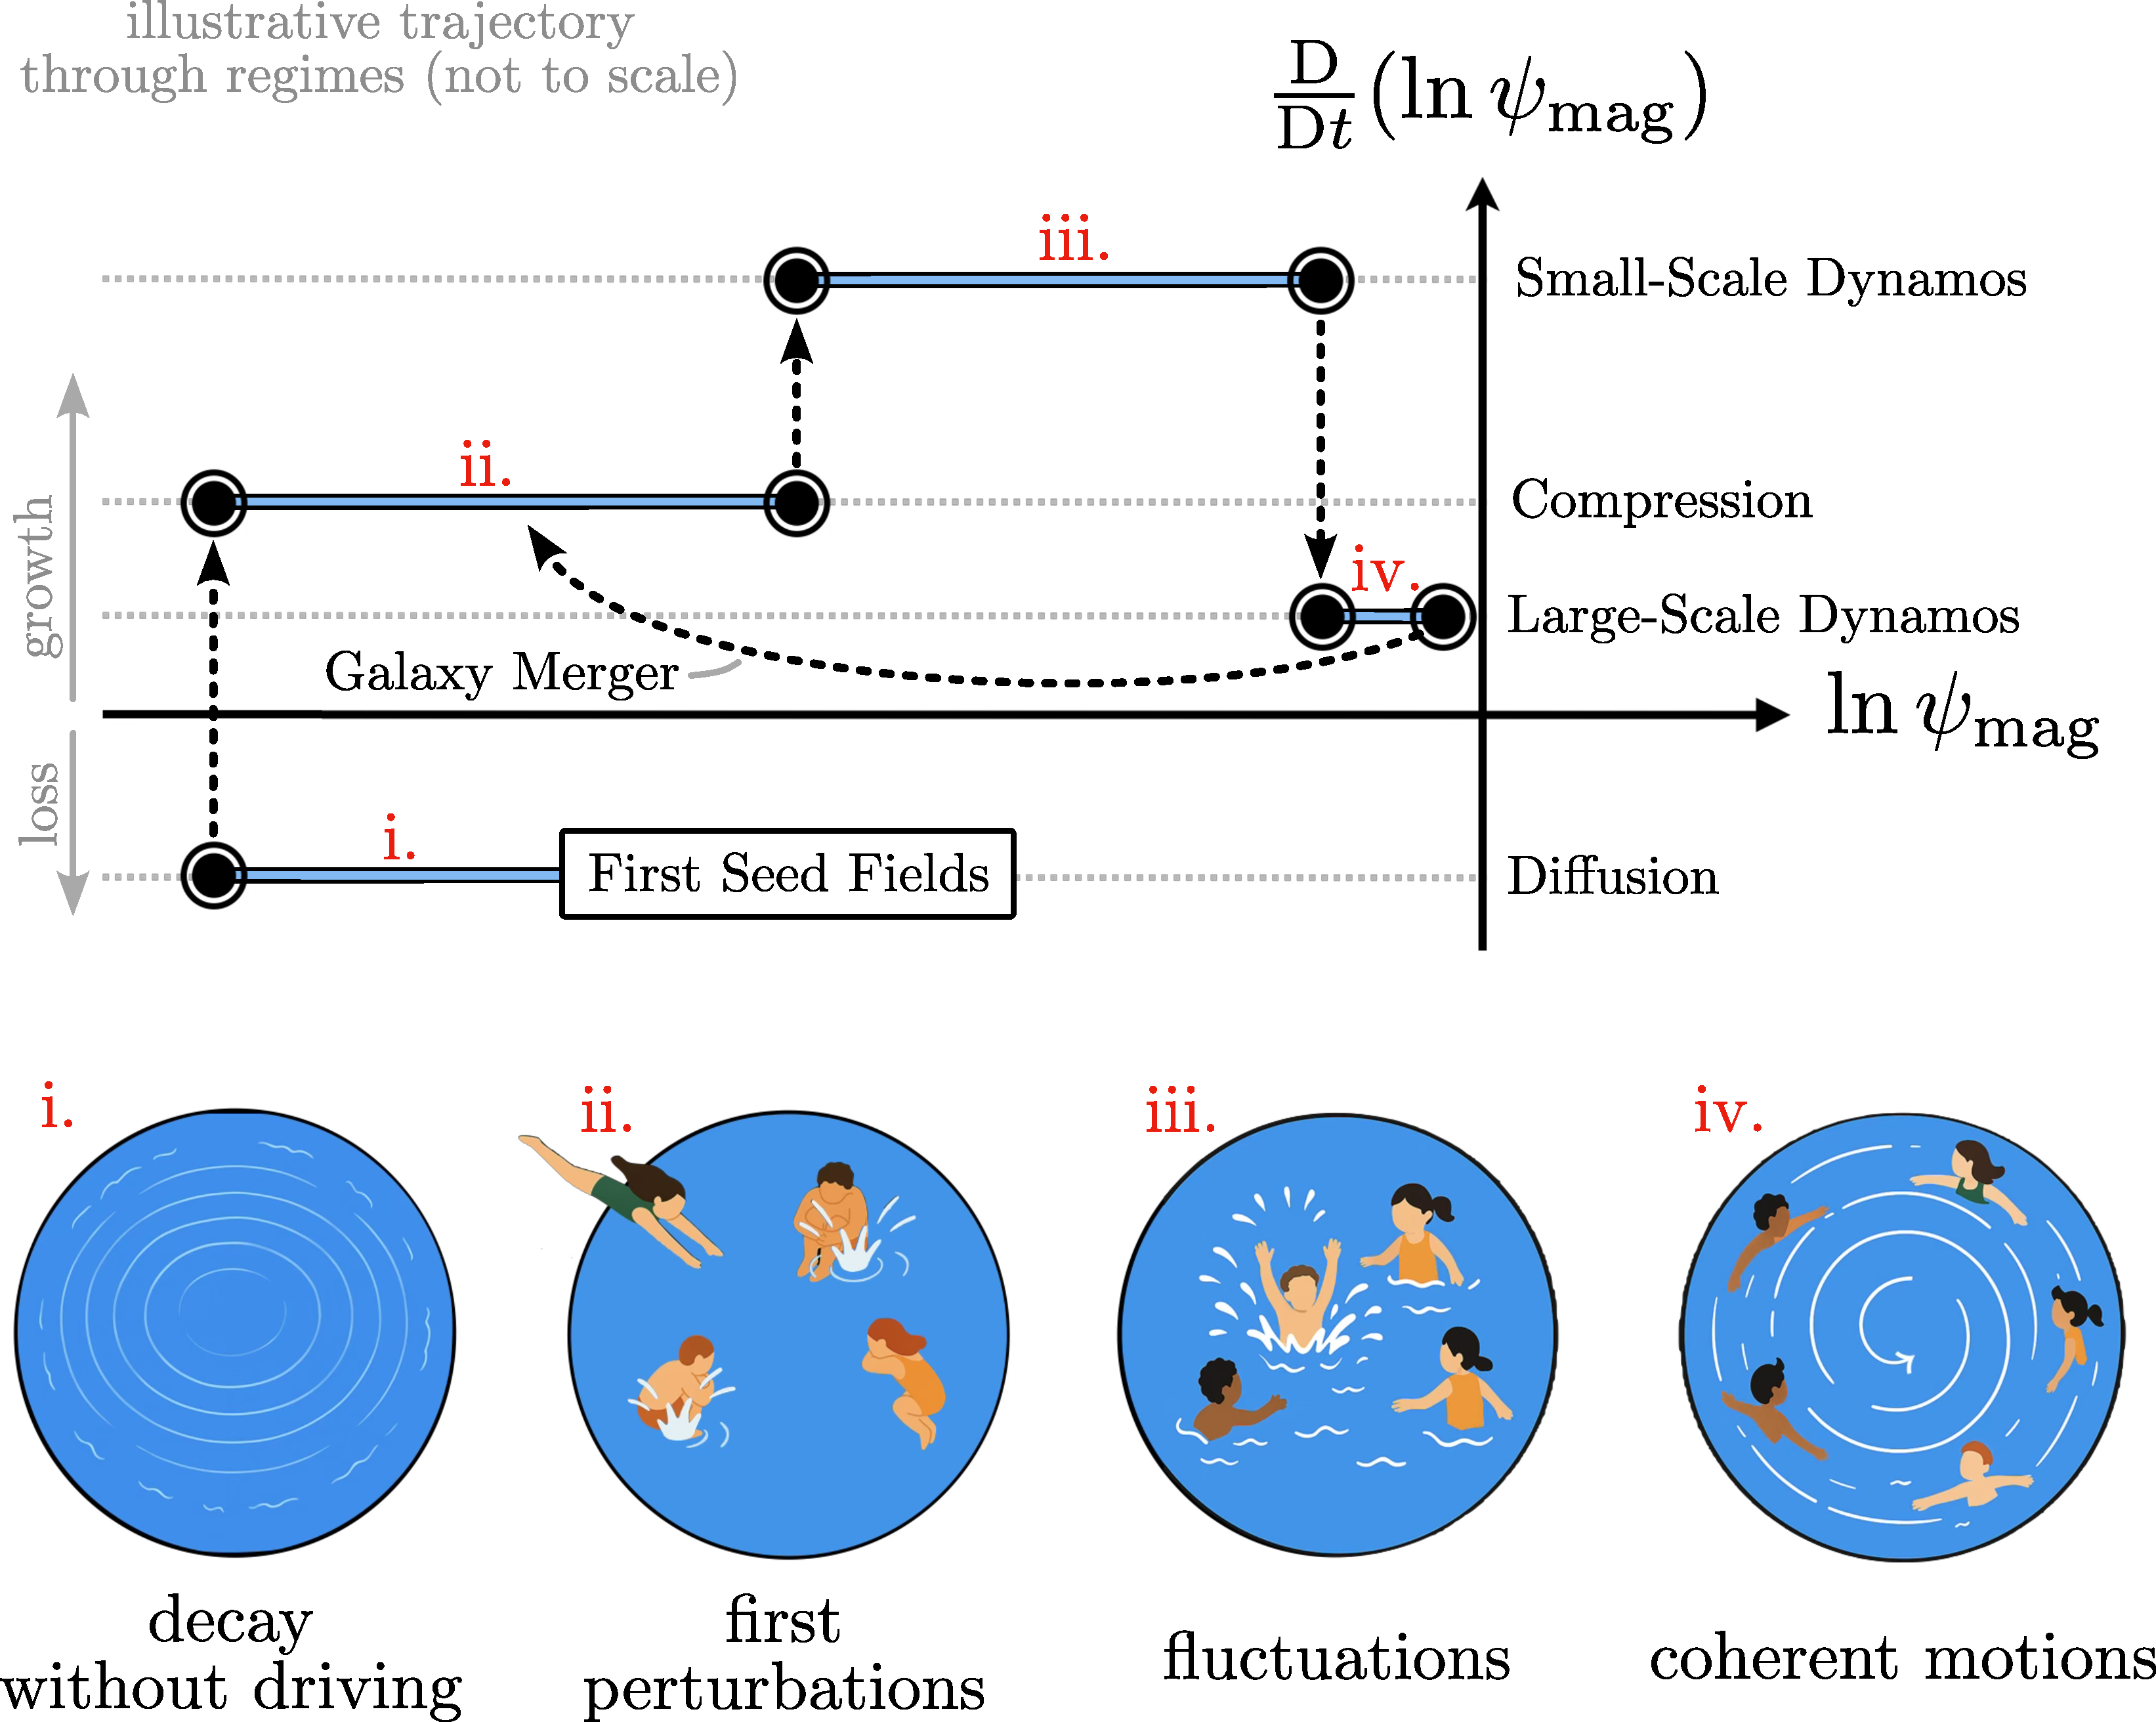
\includegraphics[width=\linewidth]{figures/introduction/dynamical.pdf}
    \caption{Schematic illustration of magnetic evolution channels (top), shown in terms of the log-transformed field strength $\ln\psi_\mathrm{mag}$ and its instantaneous fractional growth rate $\mathrm{D}(\ln\psi_\mathrm{mag}) / \mathrm{D}t$, together with a pool analogy (bottom). In the analogy, water represents magnetic fields in a plasma, and waves represent magnetic energy; it is \textit{currents} in the water that direct how waves are transported. (i) in the absence of active wave generation, waves decay (diffusion); (ii) disturbances injected into the pool grow \textit{the first} waves (\S\ref{sec:modelling:magnetogenesis} and \S\ref{sec:evolve:compression}); (iii) chaotic fluctuations produce many interacting waves, with some constructive (in-phase) and some destructive (out-of-phase) contributions, yielding net growth of waves (\S\ref{sec:evolve:ssd}; this is the most efficient means to grow waves); and (iv) sustained coherent motions develop larger-scale waves (\S\ref{sec:evolve:lsd}; harder to induce in smaller pools). The numbered yellow (brick) road indicates an illustrative trajectory through these attractor channels as the flow conditions evolve (not to scale), including the possibility of returning to earlier regimes as new episodes of compression and turbulence are reintroduced.}
    \label{fig:dynamical}
\end{figure}

The velocity field to which $\mVector{b}$ is subjected in this kinematic regime is not constant through cosmic time. As a galaxy assembles, gas first collapses into haloes and filaments, with radiative cooling and feedback driving the interstellar medium into a turbulent, multiphase state, and, in large Milky Way-like galaxies, long-lived rotation develops a coherent disc. Moreover, for large galaxies like our Milky Way, this path is not travelled just once. Instead, galaxy assembly happens through repeated mergers, which reintroduce strong compression and turbulence, and disrupt coherent rotation-driven structures, pushing the magnetic system back toward earlier flow conditions. Each epoch of magnetic field evolution reshuffles which terms in \autoref{eqn:mhd:momentum} and \autoref{eqn:mhd:induction} dominate, and moves the field onto different evolutionary channels. In \autoref{fig:dynamical} we summarise these channels and the transitions between them. In the remainder of this section we describe these channels in turn, beginning with diffusion (\S\ref{sec:evolve:decay}) and compression (\S\ref{sec:evolve:compression}), before turning to small-scale and large-scale dynamo action (\S\ref{sec:evolve:ssd} and \S\ref{sec:evolve:lsd}, respectively).

\subsubsection{Diffusion}
\label{sec:evolve:decay}

One of the first things one should notice about the induction equation, \autoref{eqn:mhd:induction}, is that it contains two competing terms. The first is inductive stretching, which couples magnetic fields to the flow, and, in the ideal limit ($\eta \to 0$), leaves them to advect flux-frozen\footnote{
    For an arbitrary material surface $\mSurface(t)$ advecting with velocity $\mVector{\chi}$, the Leibniz-Reynolds transport theorem gives
    \begin{align}
    \mppFrac{}{t} \int_{\mSurface(t)} \mVector{\xi} \cdot\mdd\mVector{S}
        &= \int_{\mSurface(t)} \sbrac{
                \mppFrac{\mVector{\xi}}{t}
                - \nabla\times(\mVector{\chi}\times\mVector{\xi})
            }\cdot\mdd\mVector{S}
        .
    \end{align}
    From this statement, it then follows that if $\mVector{\xi}$ evolves according to $\mpp_t\mVector{\xi} = \nabla\times(\mVector{\chi}\times\mVector{\xi})$, then its flux through any material surface is conserved and its topology is frozen into the medium. This condition is satisfied for ideal MHD, since $\mVector{\xi} = \mVector{b}$ obeys this induction form with $\mVector{\chi} = \mVector{u}$.
    \label{fnote:frozen}
} in the gas. The second term is diffusion, which is the inevitable consequence of real plasmas not being perfectly conducting ($\eta$ remains finite). Diffusion provides the default evolutionary channel whenever a flow does not continually regenerate magnetic structure, with the magnetic Reynolds number ($\mRem$; \autoref{defn:Rem}) providing a useful metric for when diffusion can compete with induction on a given scale. In many astrophysical environments $\mRem \gg 1$ on the largest coherent scales, but as the field is driven into smaller-scale structure, gradients sharpen and diffusion can become dynamically important.

The consequence of this is that, unless there exists a flow to stretch and produce magnetic structure, diffusion will act to remove it. In particular, this happens when $\mVector{u} \approx \mVector{0}$, or in the special case where $\mVector{u}\parallel\mVector{b}$, the induction term turns off. In these limits, \autoref{eqn:mhd:induction} reduces to a diffusion equation (assuming $\eta$ constant in space),
\begin{align}
    \mDDFrac{\mVector{b}}{t}
        \sim \eta \nabla^2 \mVector{b}
    .
\end{align}
Magnetic fields therefore decay through resistive diffusion on a characteristic timescale
\begin{align}
    t_\eta
        \sim \frac{\ell_0^2}{\eta}
        \sim \mRem \frac{\ell_0}{u_0}
    .
\end{align}

For the Earth's magnetic field, which is associated with convective motions on $\ell_0 \sim 3\times 10^8~\mathrm{cm}$ in the liquid outer core, with diffusivity $\eta \sim 10^4 \,\mathrm{cm}^2 \,\mathrm{s}^{-1}$, this predicts a decay time of $t_\eta \sim 3 \times 10^5~\mathrm{yr}$ \citep{choudhuri1998physics}, which is much shorter than the age of the Earth. This field, therefore, cannot be a fossil from magentogenesis, since any field produced alongside the Earth would have decayed by now.

If we make a similar estimate for galactic magnetic fields, we instead predict a decay time that is significantly longer than the age of the Universe. At first, one may interpret this to mean that diffusion is not relevant for galactic fields, but this conclusion is misinformed. Unlike the comparatively coherent flows relevant for the Earth, interstellar flows are not coherent. Gas in the ISM is continually stirred by supernovae and violent outflows, which generate sharp gradients and thin current layers on small scales where dissipation becomes more efficient. In this regime, decay is not well described by smooth Ohmic diffusion, which predicts $\psi_\mathrm{mag} \propto \exp(-t/t_\eta)$. Instead, the field is actively reorganised by nonlinear dynamics\footnote{
    I refer the interested reader to \citet{schekochihin2022mhd} Section~12 for a thorough review.
}, with magnetic energy selectively decayed through the formation and reconnection of small-scale structures, even at very large $\mRem$, yielding dynamical decay $\psi_\mathrm{mag} \propto t^{-p}$ with $p \sim \mathcal{O}(1)$ \citep[see \eg][]{hosking2021reconnection}. Thus magnetic erosion in the ISM is far more efficient than the naive estimate would suggest \citep{brandenburg2025turbulent}, and the presence of magnetic structure throughout the ISM therefore leads to the same conclusion as magnetic fields here on Earth, namely that it requires sustained induction.

\subsubsection{Compression}
\label{sec:evolve:compression}

Structure formation provided the first route for seed fields to grow. As baryons collapsed into the first bound objects, converging flows concentrated magnetic flux and amplified $\psi_\mathrm{mag}$. This follows directly from \autoref{eqn:mhd:induction} in the ideal (flux-frozen; see Footnote~\ref{fnote:frozen}) limit, rewritten in Lagrangian form,
\begin{align}
    \mDDFrac{\mVector{b}}{t}
        = (\mVector{b}\cdot\nabla) \mVector{u}
            - (\nabla\cdot\mVector{u}) \mVector{b}
    .
\end{align}
The continuity equation can also be rewritten in this form,
\begin{align}
    \frac{D\rho}{Dt}
        = -\rho \, (\nabla\cdot\mVector{u})
    ,
\end{align}
from which it follows that
\begin{align}
    \mDDFrac{}{t} \rfrac{\mVector{b}}{\rho}
        = \frac{1}{\rho} \mDDFrac{\mVector{b}}{t}
            - \frac{\mVector{b}}{\rho^2} \mDDFrac{\rho}{t}
        = \rbrac{\frac{\mVector{b}}{\rho}\cdot\nabla} \mVector{u}
    ,
\end{align}
and we learn that changes in $\mVector{b} / \rho$ can only arise from velocity gradients along $\mVector{b}$. Compression along $\mVector{b}$ does not change the field strength, whereas compression in directions perpendicular to $\mVector{b}$ concentrates magnetic flux and increases the magnetic field-line density.

For isotropic spherical collapse this implies $b \propto \rho^{2/3}$, and thus $\psi_\mathrm{mag} \propto \rho^{4/3}$, with
\begin{align}
    \mDDFrac{(\ln\psi_\mathrm{mag})}{t}
        = \frac{4}{3} \mDDFrac{(\ln\rho)}{t}
        = -\frac{4}{3} \nabla\cdot\mVector{u}
    .
\end{align}
Ultimately, this growth ends once thermal pressure, turbulent motions, and eventually magnetic stresses provide support against gravity. Turbulent fluctuations, however, can nevertheless continue to amplify $\psi_\mathrm{mag}$, as we will show in the next two sections.

\subsubsection{Large Scale Dynamos}
\label{sec:evolve:lsd}

\S\ref{sec:evolve:decay} revealed a key asymmetry between hydrodynamic and MHD systems: once $\psi_\mathrm{mag} > 0$, resistive diffusion provides an unavoidable channel for magnetic energy to be removed, whereas in hydrodynamics there is no analogous field that decays simply by existing. For systems like galaxies, stars, and planets, where we see magnetic fields in stable, long-lived states, the question then becomes what conditions support them. Diffusion provides one side of the answer, and growth via induction provides the other. However, anti-dynamo theorems by \citet{cowling1933magnetic} and \citet{zil1957magnetic} showed that only some fluid motions can produce dynamos; they ruled out both axisymmetric and purely planar (two-dimensional) flows. The takeaway, then, is that we should not expect overly simple, effectively two-dimensional, or highly symmetric flows to support persistent $\psi_\mathrm{mag} > 0$. Sustained magnetism requires flows with enough geometric complexity to continually regenerate the components of the field that diffusion erodes. Since Cowling and Zel'dovich, many possible dynamo scenarios have been identified (see the recent excellent reviews by, \eg \citealt{rincon2019dynamo} and \citealt{brandenburg2023galactic}). Here we focus on the standard mean-field picture relevant for Milky Way-like galaxies, and (following similar arguments in \eg \citealt{choudhuri1998physics} and \citealt{rincon2019dynamo}) show how it can generate and sustain a large-scale magnetic field.

In galaxies, radio synchrotron observations reveal magnetic structure on a wide range of scales. Polarised emission traces an ordered component that is coherent across the disc on $L \sim \mathrm{kpc}$ scales, while Faraday rotation measures indicate the presence of fluctuations on smaller $\ell_0 \sim 100 \mathrm{pc}$ scales. It then, perhaps, feels natural to decompose the galactic magnetic field into a large-scale mean component $\bar{\mVector{b}}$, describing the component of the field coherent on galactic scales $L$, and a fluctuating component $\delta\mVector{b}$, for the small-scale fluctuations about this mean on scales $\ell_0$, where $\ell_0 \ll L$. We can do the same decomposition for the velocity field, $\mVector{u} = \bar{\mVector{u}} + \delta\mVector{u}$, which, when substituted into \autoref{eqn:mhd:induction} and averaged over intermediate scales $\ell \in [\ell_0, \,L]$ (using Reynolds averaging rules), yields
\begin{align}
    \overline{\mppFrac{\mVector{b}}{t}}
        =  \mppFrac{\bar{\mVector{b}}}{t}
        = \mCurl{\rbrac{
            \bar{\mVector{u}} \times \bar{\mVector{b}}
            + \overline{\delta\mVector{u} \times \delta\mVector{b}}
            - \eta \mCurl{\bar{\mVector{b}}}
        }}
        . \label{eqn:lsd:average}
\end{align}
The companion evolution equation for magnetic fluctuations, is then
\begin{align}
    \mppFrac{(\delta\mVector{b})}{t}
        &= \mppFrac{\mVector{b}}{t} - \mppFrac{\bar{\mVector{b}}}{t} \\
        &= \mCurl{\rbrac{
            \bar{\mVector{u}}\times\delta\mVector{b}
            + \delta\mVector{u}\times\bar{\mVector{b}}
            + \delta\mVector{u}\times\delta\mVector{b}
            - \overline{\delta\mVector{u}\times\delta\mVector{b}}
            - \eta \mCurl{\delta\mVector{b}}
        }}
    . \label{eqn:lsd:delta:full}
\end{align}
Notice that $\bar{\mVector{b}}$ does not only evolve based on the large-scale features of the system, but also on the fluctuations, $\delta\mVector{b}$ and $\delta\mVector{u}$, and, importantly, the average correlation between them, $\overline{\delta\mVector{u}\times\delta\mVector{b}}$. To put forward a description for how $\bar{\mVector{b}}$ can then be generated in a galaxy, we adopt typical approximation that the contribution to this correlation is dominated by the part of $\delta\mVector{b}$ produced by turbulent distortions of the slowly varying $\bar{\mVector{b}}$. In this picture, the self-interaction of fluctuations, $ \delta\mVector{u}\times\delta\mVector{b} - \overline{\delta\mVector{u}\times\delta\mVector{b}} $, is, to first order, unimportant for the component of $\delta\mVector{b}$ that feeds back into $\bar{\mVector{b}}$. Neglecting these terms reduces \autoref{eqn:lsd:delta:full} to
\begin{align}
    \mppFrac{(\delta\mVector{b})}{t}
        \approx \mCurl{\rbrac{
            \underbrace{
                \bar{\mVector{u}}\times\delta\mVector{b}
            }_\text{mean flow advects $\delta\mVector{b}$}
            + \overbrace{
                \delta\mVector{u}\times\bar{\mVector{b}}
            }^\text{\shortstack{mean field is imprinted\\ onto $\delta\mVector{b}$}}
            - \underbrace{
                \eta \mCurl{\delta\mVector{b}}
            }_\text{diffusion damps $\delta\mVector{b}$}
        }}
    , \label{eqn:lsd:delta:reduced}
\end{align}
and motivates a closure for the average electromotive force in \autoref{eqn:lsd:average}.

Since $\bar{\mVector{b}}$ varies on scales larger than the fluctuating fields, we can approximate $\overline{\delta\mVector{u} \times \delta\mVector{b}}$ via a gradient expansion of $\bar{\mVector{b}}$, which, in index notation, takes the form
\begin{align}
    (\overline{\delta\mVector{u} \times \delta\mVector{b}})_{i}
        = \alpha_{ij} \bar{b_j} - \pi_{ijk} \mppFrac{\bar{b_j}}{x_k} + \cdots
    .
\end{align}
Here, $\alpha_{ij}$ and $\pi_{ijk}$ are transport coefficients that encode the net effect of fluctuations (\eg stratification, and angular velocity). If we assume that $\delta\mVector{u}$ is approximately homogeneous and isotropic, then these tensors simplify considerably to $\alpha_{ij} = \alpha \delta_{ij}$ and $\pi_{ijk} = \eta_{\delta u} \epsilon_{ijk}$, and the expansion simplifies to
\begin{align}
    \overline{\delta\mVector{u} \times \delta\mVector{b}}
        \approx \alpha \bar{\mVector{b}} - \eta_{\delta u} \mCurl{\bar{\mVector{b}}}
    ,
\end{align}
where $\eta_{\delta u}$ is (turbulent) mixing induced diffusion\footnote{
    Consider a sugar cube in a cup. Left unstirred, it dissolves slowly through molecular diffusion, which can take many days. This process is largely inefficient, because the cube quickly surrounds itself with a sugar-rich boundary layer that throttles diffusion. If the water is stirred, however, this layer is advected away and replaced by fresh fluid, which allows the cube to dissolve more efficiently. Turbulent mixing enhances diffusion in the same way.
}. This only holds in the regime where $\delta b \ll \delta u$, but when $\delta b \sim \delta u$, then $\alpha$ will also have a dependence on $\mVector{b}$ \citep[see \eg][]{cattaneo1996nonlinear}.

With this, we now have an evolution equation for $\bar{\mVector{b}}$ in a system where a slowly varying $\bar{\mVector{u}}$ interacts with $\delta\mVector{u}$. In the context of galactic flows, the large scale flow is dominated by differential rotation, best described in cylindrical coordinates $\bar{\mVector{u}} = r \Omega(r) \hat{\mVector{\phi}}$. In this system, the evolution equation becomes
\begin{align}
    \mppFrac{\bar{\mVector{b}}}{t}
        \approx \mCurl{\rbrac{
            \overbrace{
                r \Omega \rbrac{
                    \bar{b}_z \mVectorUnit{r}
                    - \bar{b}_r \mVectorUnit{z}
                }
            }^\text{differential rotation}
            + \underbrace{
                \alpha \bar{\mVector{b}}
            }_\text{kinetic helicity}
            - \overbrace{
                (\eta + \eta_{\delta u}) \mCurl{\bar{\mVector{b}}}
            }^\text{diffusion}
        }}
    ,
\end{align}
which highlights the important, and combined role that differential rotation plays along with kinetic helicity. Differential rotation plays the role of winding magnetic field lines around the rotation axis, producing a toroidal component\footnote{
    Since $\mpp_t \bar{b}_\phi \sim r \bar{b}_r \mppFrac{\Omega}{r}$, any $\bar{b}_r$ component of $\bar{\mVector{b}}$ is ultimately stretched by differential rotation into something toroidal, $\bar{b}_\phi$.
    \label{fnote:lsd:omega}
} about the disc, which, in the absence of helicity, $\alpha \approx 0$, does not lead to a self-sustaining dynamo. This is because differential rotation cannot recover poloidal fields once $\bar{b}$ is primarily $\bar{b}_\phi$, and so the large-scale field ultimately erodes away through diffusion (in the same spirit as Cowling's theorem). Helicity importantly regenerates poloidal fields from toroidal ones\footnote{
    For an axisymmetric disc $(\mpp_\phi = 0)$, the $\alpha$-term converts toroidal fields $\bar{b}_\phi$, back into poloidal ones. To see this, recall that the radial and vertical components of the curl in cylindrical coordinates are
    \begin{align}
    \sbrac{\mCurl{(\alpha\bar{\mVector{b}})}}_r
        = -\mppFrac{(\alpha \bar{b}_\phi)}{z}
    \qquad\mbox{and}\qquad
    \sbrac{\mCurl{(\alpha\bar{\mVector{b}})}}_z
        = \frac{1}{r}\mppFrac{}{r}\sbrac{r \alpha\bar{b}_\phi}
    ,
    \end{align}
    respectively. Therefore, $\mCurl{(\alpha\bar{\mVector{b}})}$ generates $\bar{b}_r$ and $\bar{b}_z$ from gradients of $\bar{b}_\phi$.
    \label{fnote:lsd:alpha}
}, which replenishes poloidal fields for differential rotation to wind up. Together, these two processes couple to form the $\alpha$-$\Omega$ dynamo, capable of sustaining coherent galactic fields.

One way to estimate how efficiently this process can operate is to consider how quickly the $\Omega$-effect generates toroidal fields, and the $\alpha$-effect then regenerates poloidal fields (\ie how quickly the dynamo process passes through the steps of see the schematic in \autoref{fig:galaxy}). We do so by recalling that we had assumed $\bar{\mVector{b}}$ varies on scales of the system $L$, so the radial contribution of the $\alpha$-term in \autoref{eqn:lsd:average} can be estimated to be
\begin{align}
    \mppFrac{\bar{b}_r}{t}
        = \sbrac{\mCurl{(\alpha \bar{\mVector{b}})}}_r
        \sim \frac{\alpha}{L} \bar{b}_\phi
    .
\end{align}
Taking a second time derivative and substituting the rate at which the $\Omega$-term winds fields (see Footnote~\ref{fnote:lsd:omega}), gives
\begin{align}
    \mppFrac{^2 \bar{b}_r}{t^2}
        \sim \frac{\alpha}{L} \mppFrac{\bar{b}_\phi}{t}
        \sim \frac{\alpha}{L} \rbrac{r \mppFrac{\Omega}{r}} \bar{b}_r
    ,
\end{align}
which reveals an estimate for the characteristic growth rate,
\begin{align}
    \gamma
        \sim \sqrt{\frac{\alpha}{L} r \mAbs{\mppFrac{\Omega}{r}}}
    .
\end{align}
This growth rate must compete against turbulent diffusion, which damps the mean field at a rate $\sim (\eta + \eta_{\delta u}) / L^2$, with net growth only possible when
\begin{align}
    \sqrt{\alpha L^3 r \mAbs{\mppFrac{\Omega}{r}}}
        \gtrsim \eta + \eta_{\delta u}
    ,
\end{align}
where this excitation condition is usually expressed in terms of a ``dynamo number''
\begin{align}
    \mathcal{D}
        \equiv \frac{
                L^3 \alpha r \mAbs{\mpp_r \Omega}
            }{
                (\eta + \eta_{\delta u})^2
            }
    ,
\end{align}
with large-scale growth expected when $\mathcal{D} \gtrsim \mathcal{O}(1 - 10)$.

\begin{figure}
    \centering
    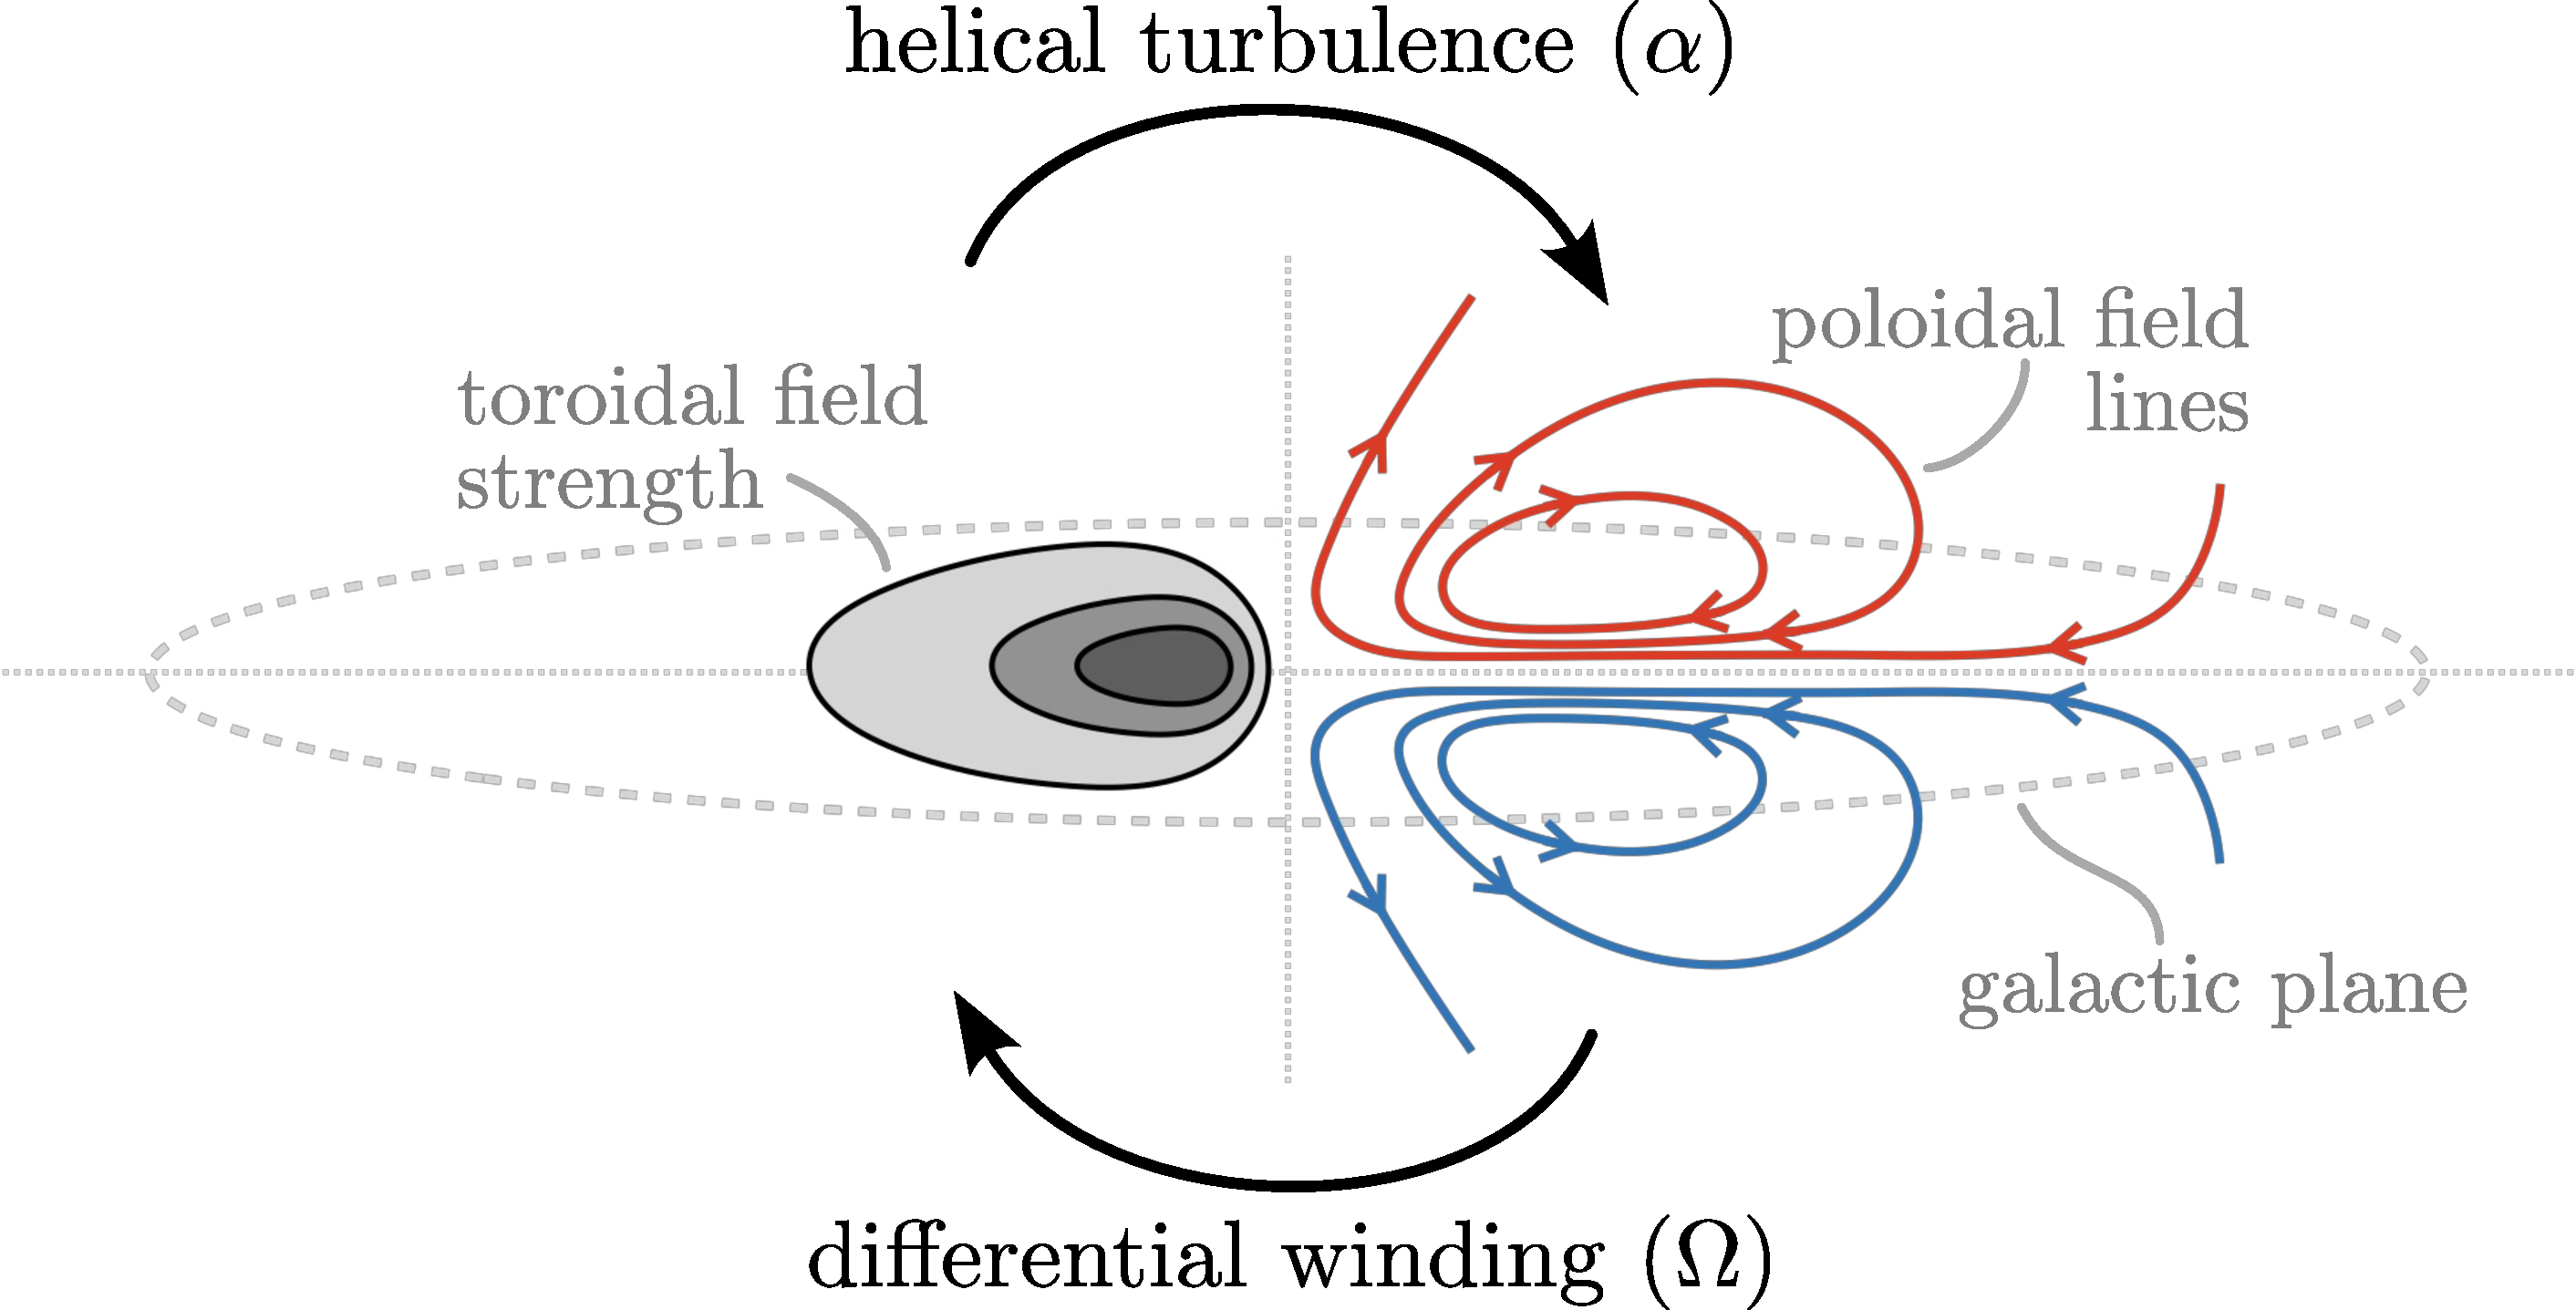
\includegraphics[width=0.9\linewidth]{figures/introduction/galaxy.pdf}
    \caption{Schematic of an $\alpha-\Omega$ dynamo operating in a galaxy, adapted from \citet{klein2014galactic}. The large-scale galactic magnetic field is decomposed into a toroidal component (left; wrapped around the disc's rotation axis) and a poloidal component (right; field lines thread the disc and halo). Differential rotation winds poloidal flux into toroidal flux (the $\Omega$ effect), and helical turbulence regenerates poloidal fields from toroidal ones (the $\alpha$ effect). Together, these two processes create a closed feedback loop that can generate and maintain coherent large-scale structure against turbulent and resistive diffusion.}
    \label{fig:galaxy}
\end{figure}

In large spiral galaxies, where differential rotation is both strong and coherent on $\sim \mathrm{kpc}$ scales, it is easy for this condition to be satisfied. For example, \citet{ntormousi2020dynamo} used direct numerical simulations to show that an $\alpha$-$\Omega$ LSD was active in a Milky Way-like galaxy, where an ordered field was measured to grow over $\sim 0.5 \,\mathrm{Gyr}$. This growth is consistent with our estimate for $\gamma$ above, which, for a typical spiral-galaxy, where $L \sim 10 \,\mathrm{kpc}$, $\alpha \sim 1 \,\mathrm{km} \,\mathrm{s}^{-1}$, and $r |\mdd \Omega / \mdd r| \sim \Omega \sim 30 \,\mathrm{km} \,\mathrm{s}^{-1} \,\mathrm{kpc}^{-1}$, gives $\gamma \approx 2\times 10^{-3} \,\mathrm{Myr}^{-1}$. As we discuss in the next section, this rate of amplification is notably slower than small-scale dynamo growth, which is driven by the same turbulent motions. The LSD is therefore unlikely to be the sole (or primary) mechanism for galactic magnetic field strengths, even in large spiral galaxies. The role of the LSD is even more questionable in smaller galaxies, where differential rotation is weaker and often less coherent. In these systems, the $\Omega$-effect becomes inefficient, and diffusion can more easily overwhelm large-scale growth, so an $\alpha$-$\Omega$ LSD struggles to explain the inferred field amplitudes. Nonetheless, the LSD provides a natural route to generating the coherent large-scale structure observed in spiral discs.

% Parker (1955) phenomenology [Rincon 4.2.2]. Steenbeck, Krause \& Radler (1966), Vainshtein (1970), Moffatt (1970) [Rincon 4.3].

\subsubsection{Small Scale Dynamos}
\label{sec:evolve:ssd}

A key element of the $\alpha$-$\Omega$ dynamo is the role played by velocity fluctuations, $\delta\mVector{u}$. While they contribute an important ingredient for amplifying large-scale magnetic fields via their role in the net correlation $\overline{\delta\mVector{u}\times\delta\mVector{b}}$ in \autoref{eqn:lsd:average}, they can also drive local magnetic amplification on the scales of the fluctuations themselves. Here we will focus on these fluctuations, and show that they produce the fastest, most efficient, and readily available scenario for magnetic amplification.

Working in a locally comoving frame where $\bar{\mVector{u}} \approx \mVector{0}$, we will, for notational convenience, write $\mVector{u} \equiv \delta\mVector{u}$ and $\mVector{b} \equiv \delta\mVector{b}$, and drop the $\delta$ symbol. Local amplification  then follows from the interactions of fluctuating velocity gradients with the magnetic field, where only certain interactions are productive. To see which motions grow the magnetic energy density, consider
\begin{align}
    \mDDFrac{\psi_\mathrm{mag}}{t}
        = \frac{1}{4\pi} \rbrac{
                \overbrace{
                    \mVector{b}\otimes\mVector{b}:\nabla\otimes\mVector{u}
                }^\text{\shortstack{stretching\\ + compression}}
                - \underbrace{
                    b^2 \rbrac{\nabla\cdot\mVector{u}}
                }_\text{compression}
                - \overbrace{
                    \eta \,\mVector{b}\cdot\nabla^2\mVector{b}
                }^\text{diffusion}
            }
        \label{eqn:induction:lagrangian}
    .
\end{align}

Using index notation for the moment, the first term $ b_i b_j \mpp_j u_i $ measures the component of the velocity gradient projected along the local field direction, which contains both strain and compressive contributions. Following \citet{beattie2023bulk}, it is useful to decompose the velocity gradient tensor into $\mpp_j u_i = S_{ij} + R_{ij} + C_{ij}$, where
\begin{align}
    S_{ij}
        &\equiv \frac{1}{2} \rbrac{\mpp_j u_i + \mpp_i u_j}
            - \frac{1}{3} (\mpp_k u_k) \delta_{ij}
        & \mbox{(strain)} \\
    R_{ij}
        &\equiv \frac{1}{2} \rbrac{\mpp_j u_i - \mpp_i u_j}
        & \mbox{(rotation)} \\
    C_{ij}
        &\equiv \frac{1}{3} (\mpp_k u_k) \delta_{ij}
        . & \mbox{(compression)}
\end{align}
This split reveals the three fundamental types of local actions that a flow can perform on a fluid element, namely, volume-preserving deformation $\mTensor{S}$, rigid rotation $\mTensor{R}$, and isotropic volume change $\mTensor{C}$ (with compression or expansion set by the sign of $\theta \equiv \mathrm{Tr}(\mTensor{C})$), respectively.

The first model to demonstrate how fluctuating velocity fields can drive magnetic amplification was put forward by \citet{moffatt1961amplification} for incompressible flows ($\theta = 0$), and later extended by \citet{zel1984kinematic} to flows with finite correlation times. It is popularly referred to as the \textit{stretch-twist-fold} mechanism, and is best viewed as a pedagogical picture that explains how magnetic amplification is possible through a small set of repeatable, local deformations acting on a magnetic flux tube. In the language of \citet{beattie2023bulk} (see also \citealt{schekochihin2002spectra, seta2021saturation, sur2024role}), these actions map naturally onto the strain and rotation tensors, $\mTensor{S}$ and $\mTensor{R}$, together with diffusion.

\begin{figure}
    \centering
    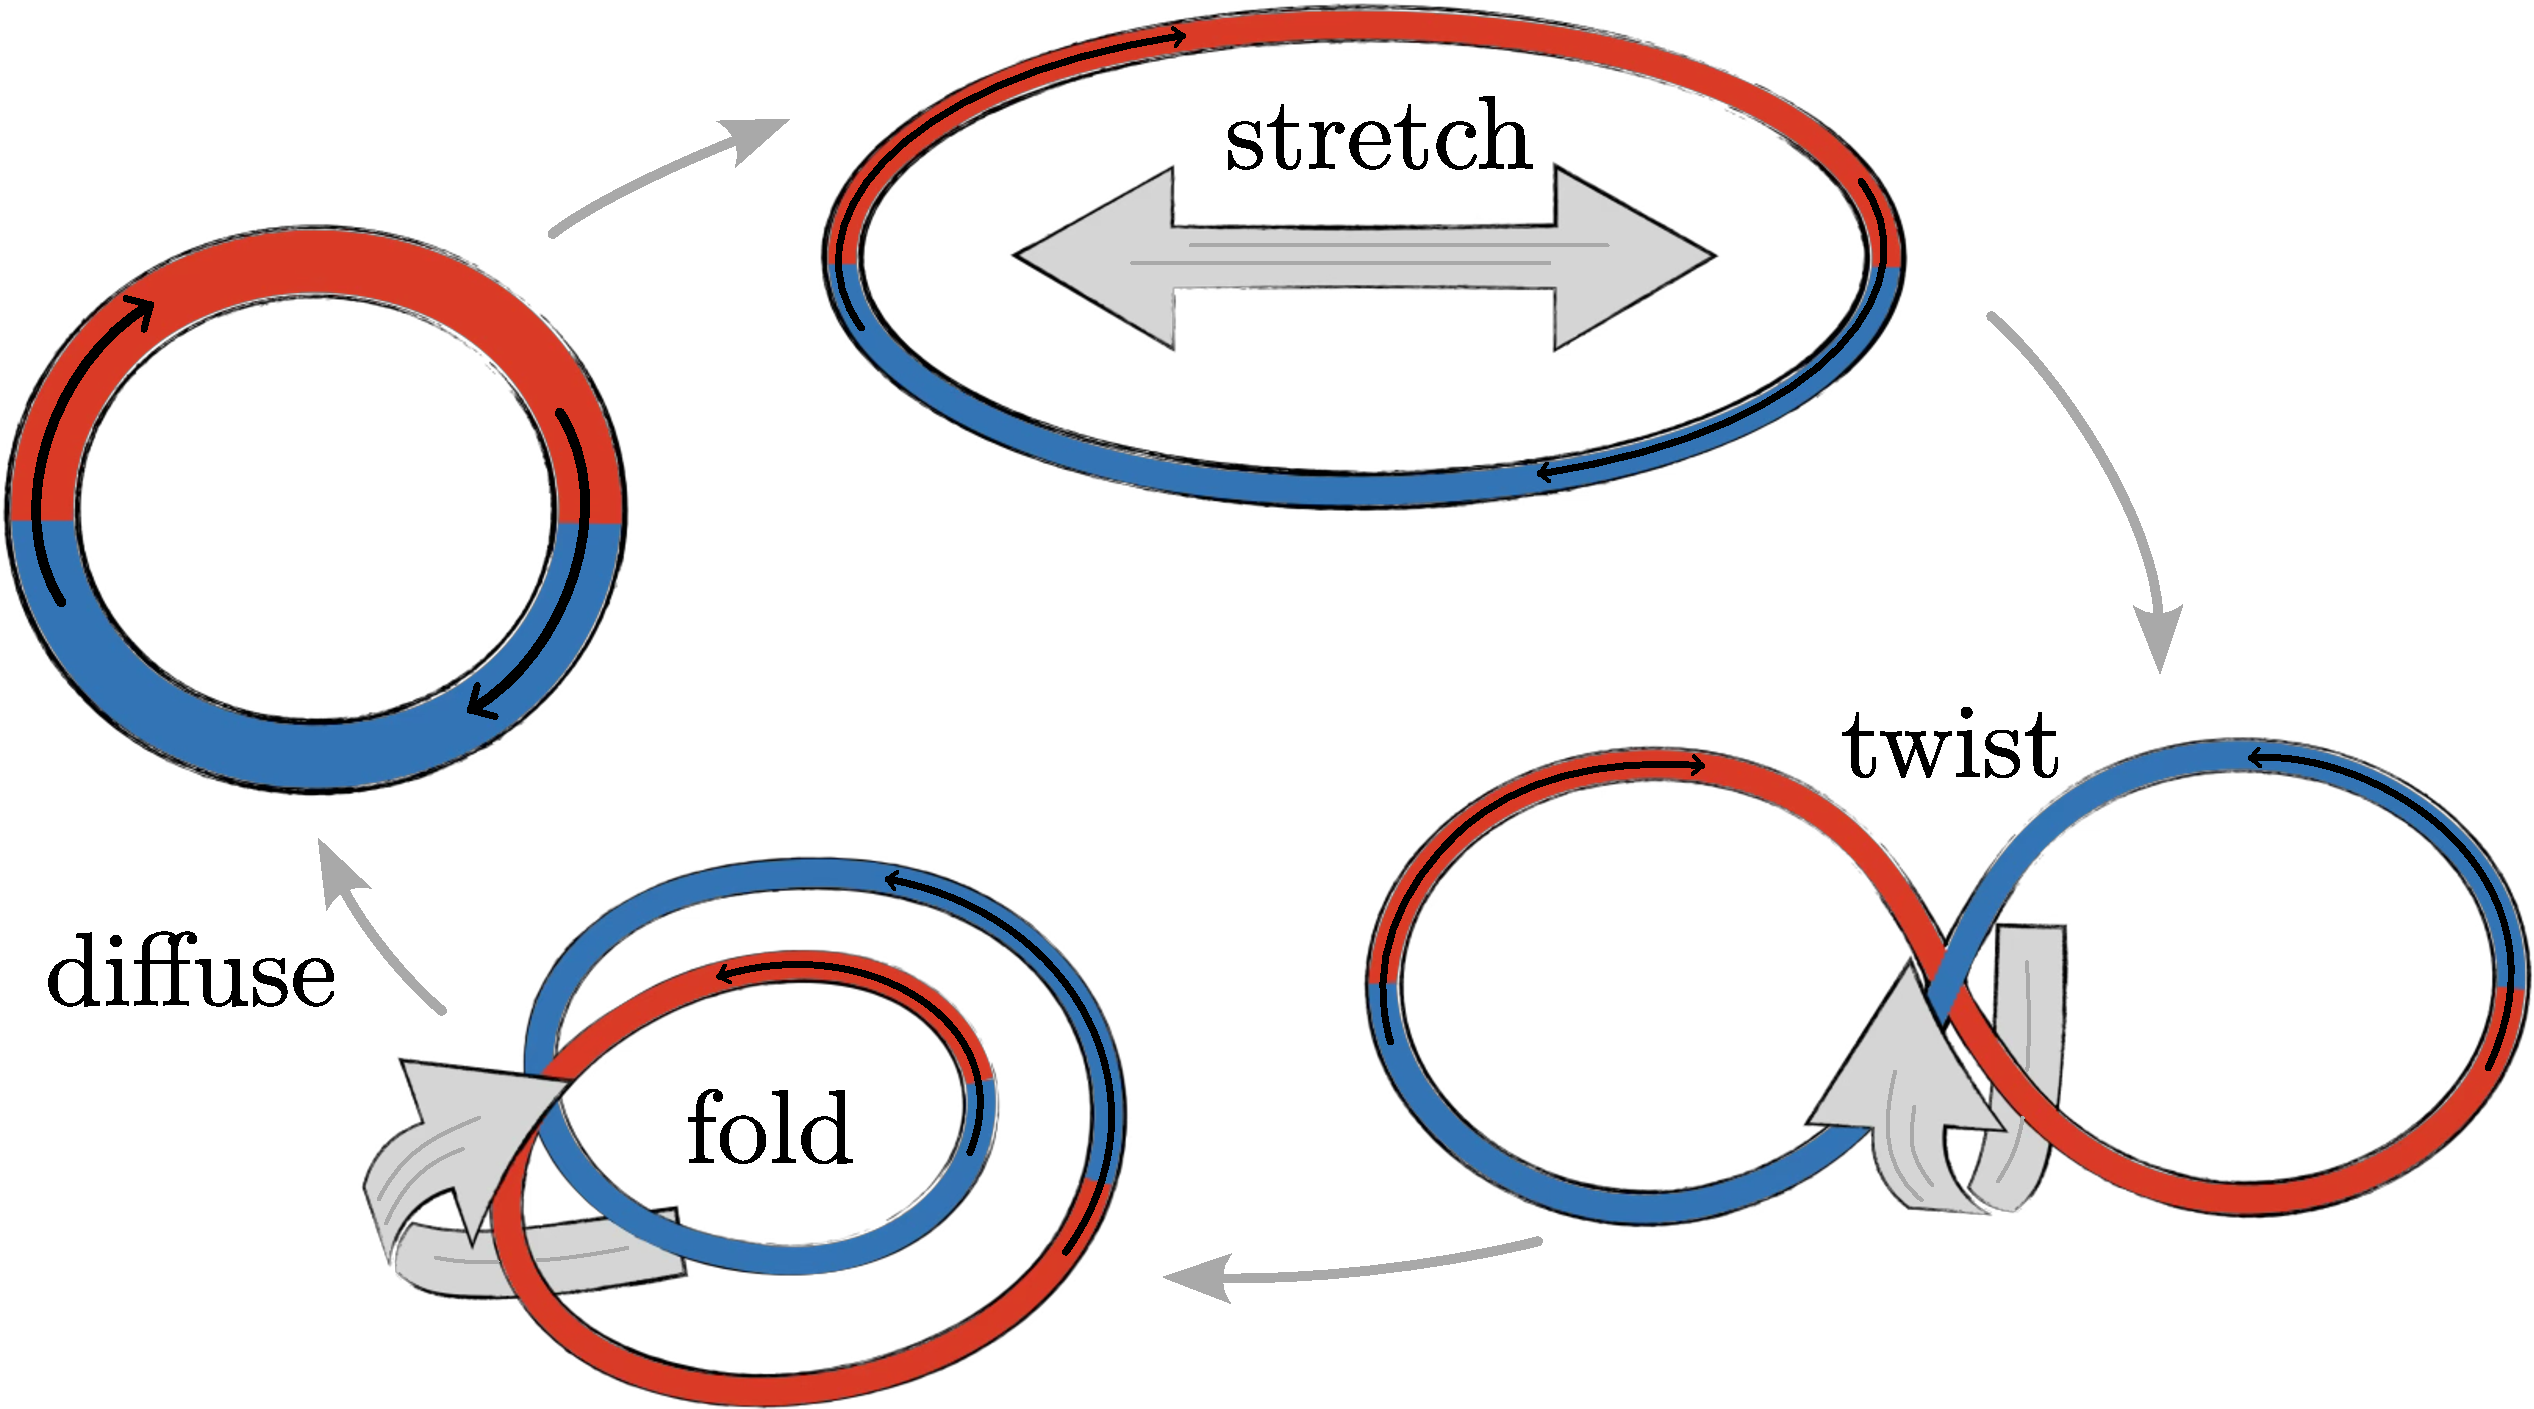
\includegraphics[width=0.8\linewidth]{figures/introduction/STF.pdf}
    \caption{Schematic of the \textit{stretch-twist-fold} (and diffuse) mechanism, adapted from \citet{rincon2019dynamo}. A closed loop of magnetic field is repeatedly (i) stretched by strain, concentrating flux into a smaller cross-section, thereby increasing magnetic energy; (ii) twisted and reoriented by rotational motions; and (iii) folded to bring segments of opposite polarity into close contact; (iv) diffusion merges the folded segments, making this cycle irreversible.}
    \label{fig:STF}
\end{figure}

Stretching is induced when strain acts along the local field direction, $\mVector{b}\otimes\mVector{b}:\mTensor{S}$, which concentrates magnetic flux into progressively thinner cross-sections and thereby increases the local magnetic energy density. Sustained growth then requires repeated stretching events, but repeated, random deformation events need not lead to monotonic amplification, since the evolution remains reversible: random stretching events may counter one-another. Rotation, while unable to change the magnetic energy density directly\footnote{
    Since $b_i b_j$ is symmetric and $R_{ij}$ is antisymmetric, $b_i b_j R_{ij} = 0$, which matches the intuition that pure rotation can reorient $\mVector{b}$ but cannot change its magnitude.
}, plays an important role by reorienting the field loop, which can lead to twisting and folding of the field. Diffusion then provides the final, essential ingredient for making this process irreversible\footnote{
    This should really be called the \textit{stretch-twist-fold-diffuse} mechanism.
}, merging the field after it has been stretched, twisted, and folded. This is summarised in \autoref{fig:STF}.

In real plasma flows, this picture should not be interpreted as a literal, coherent sequence of actions acting on a single magnetic flux tube, but instead as a statistical description of what happens to bundles of magnetic field lines as they are entrained in stochastic, often turbulent flows. \citet{kazantsev1968} successfully turned this statistical idea into a quantitative theory by deriving an evolution equation whose growing solution predicts a magnetic energy spectrum (see \citealt{rincon2019dynamo} for details) with asymptotic form
\begin{align}
    \psi_\mathrm{mag}(k, t)
        \propto \exp(\gamma t) \rfrac{k}{k_\eta}^{3/2} K_0\rfrac{k}{k_\eta}
        ,
        \label{eqn:kazantsev}
\end{align}
where $K_0$ is a Macdonald function, $k \equiv 2\pi / \ell$ is the Fourier wavenumber, $k_\eta$ is the resistive wavenumber (where $\mRem \sim 1$), and $\gamma \sim \mAve{\mVectorUnit{b}\otimes\mVectorUnit{b}:\mTensor{S}}_{\mSurface(t)}$ is the average rate of field-line stretching along advected material surfaces $\mSurface(t)$.

Although it was originally formulated for solar magnetic fields, \autoref{eqn:kazantsev} has since proven remarkably successful at predicting magnetic field statistics in turbulent systems, and, since turbulence is ubiquitous\footnote{
    The ``big power-law in the sky'' suggests turbulent velocity fluctuations span across more than six decades: from $\sim 10^4\,\mathrm{pc}$ down to $\lesssim 10^{-2}\,\mathrm{pc}$; see, \eg \citet{kalberla2019turbulent} and \citet{liu2025tiny}.
}, in astrophysical plasmas, the theory has found widespread success, including in supernova-driven, multiphase ISM simulations \citep{gent2023transition}. \citet{kulsrud1992spectrum} and \citet{schekochihin2001structure}, for example, coupled the Kazantsev \citep{kazantsev1968} framework to Kolmogorov turbulence, which led to a picture of magnetic growth where stretching becomes controlled by the fastest, and thus smallest, turbulent eddies, $\ell_\nu$ (where $\mReh \sim 1$; confirmed in, \eg \citealt{kriel2022fundamental}). This leads to growth rate $\gamma \sim 1 / t_\nu \sim u_\nu/\ell_\nu \sim (u_0 / \ell_0) \,\mReh^{1/2}$, which, in the $\mReh \gg 1$ interstellar medium predicts SSD growth on dynamical timescales $\sim \mathrm{Myr}$, which is significantly faster than the $\alpha$-$\Omega$ LSD \citep[\eg][]{gent2023transition}, though LSD efficiency can be limited by $\alpha$-quenching \citep{vishniac2001magnetic}.

The current paradigm for galactic magnetism is therefore that SSD action is essentially inevitable, and provides the most efficient route for magnetic amplification. Given its ingredients are readily available across all epochs of galaxy evolution, it believed that SSDs ultimately set the overall magnetic field strength. In galaxies that can also support an LSD, for example the $\alpha$-$\Omega$ dynamo we discussed in \S\ref{sec:evolve:lsd}, large-scale induction then acts on already amplified magnetic fields to organise them into coherent, ordered fields. This coherence is not permanent, however, since mergers can disrupt disc rotation and reintroduce strong turbulence, effectively resetting the large-scale ordering and returning the magnetic system to an SSD-dominated state until coherent rotation re-emerges.


\section{Thesis Roadmap and Remaining Lacunae}
\label{sec:intro:roadmap}

The remainder of this thesis is organised around three paper-chapters. The first two chapters are published papers, and explore aspects of SSD amplification with particular emphasis on the role of compressibility. The final chapter is a code-development paper in the final stages of preparation, wherein we implement an MHD module in a new astrophysical simulation code. Below we briefly motivate each chapter; each chapter also includes a dedicated introduction that provides further context and an overview of the relevant literature.

\uline{\S\ref{chapter:ssd-exp} focuses on kinematic SSD amplification in compressible turbulence.} While the classical Kazantsev formalism provides a quantitative description of kinematic dynamo growth, it is most often (as discussed in \S\ref{sec:evolve:ssd}) interpreted through the lens of incompressible turbulence models. Extensions beyond the incompressible limit have been developed for compressible flows \citep[\eg][]{schober2012magnetic, bovino2013turbulent}, but their consequences for the generated magnetic structures remain comparatively less explored. This matters because compressibility introduces shocks and strong density intermittency that affect how SSDs operate \citep{federrath2016magnetic}. Because shocks potentially organise magnetic fields on large scales, compressibility may help explain the $\sim \mathrm{kpc}$-scale magnetic structure inferred in young galaxies (see \S\ref{sec:what-we-see}) at epochs when LSDs are unlikely to have had time to organise coherent fields. \S\ref{chapter:ssd-exp} explores whether compressibility can indeed help resolve this tension.

\uline{\S\ref{chapter:ssd-nl} focuses on the nonlinear stage of SSD amplification}, when magnetic fields become dynamically important and begin to modify the stretching motions that amplify them. It is well understood that SSD growth is exponential in the kinematic stage, but the subsequent nonlinear evolution remains an active area of debate. While many theories make predictions for the growth rate, efficiency, and timescale of saturation, there has been a lack of systematic work to test them. These uncertainties are further exacerbated in compressible turbulence because shocks and strong intermittency introduce additional couplings. Progress has largely been limited by the fact that the nonlinear stage is transient and mediated by intermittent flows, so measurements from any single realisation are strongly stochastic. \S\ref{chapter:ssd-nl} therefore develops a statistical framework based on ensembles of simulations, designed to extract the deterministic behaviour underlying nonlinear SSD growth and to obtain measurements that can directly test proposed nonlinear theories.

Finally, \uline{\S\ref{chapter:quokka} implements a new MHD constrained-transport (CT) scheme in the \textsc{Quokka} codebase}. Following the dynamical roads discussed in \S\ref{sec:evolve:paths}, it is clear that a single, self-consistent simulation of galaxy evolution requires resolving a wide dynamic range, from $\sim 10 \,\mathrm{kpc}$ down to $\sim 10 \,\mathrm{pc}$. This has been difficult to achieve with existing CPU-based codes, but is now becoming practical with next-generation, GPU-accelerated supercomputers, which \textsc{Quokka} was developed for from its outset. Until now, however, \textsc{Quokka} has lacked an MHD module. In \S\ref{chapter:quokka} we discuss our implementation of a new CT-based scheme, and validate that it  is both accurate enough for these applications, while remaining efficient enough to scale to the required resolutions.
